\documentclass{article}%
\usepackage[T1]{fontenc}%
\usepackage[utf8]{inputenc}%
\usepackage{lmodern}%
\usepackage{textcomp}%
\usepackage{lastpage}%
%
\usepackage{amsmath}%
\usepackage{amssymb}%
\usepackage{amsfonts}%
\usepackage{graphicx}%
\usepackage{hyperref}%
\usepackage{tikz}%
\usepackage{pgfplots}%
\usetikzlibrary{math}%
\title{ITA 2027 - Física\thanks{This exam was solved and automatically generated with gpt-resolve: \url{https://github.com/lgabs/gpt-resolve}}}%
\author{claude{-}sonnet{-}5{-}5 (solver) + claude{-}sonnet{-}5{-}5 (judge)}%
\date{November 09, 2026}%
%
\begin{document}%
\normalsize%
\maketitle%
\section*{Questão 1}

\section*{Solução}

\textbf{Modelo.} Seja $\theta$ o ângulo da haste com a vertical e $r=k/k_c$. A haste é rígida e homogênea (centro de massa a $L/2$ do mancal), o sistema tem um único grau de liberdade ($\theta$) e as forças são conservativas (peso e torque elástico). Basta, então, estudar $U_{total}(\theta)$: equilíbrio onde $U'=0$; estável se $U''>0$ (mínimo) e instável se $U''<0$ (máximo).

Altura do centro de massa: $h=\dfrac{L}{2}\cos\theta$. Energia da mola torcional ($\tau_e=-k\theta$, logo $U_e=\int_0^\theta k\theta'\,d\theta'$): $\tfrac12 k\theta^2$. Assim,
\[
U_{total}(\theta)=\frac{MgL}{2}\cos\theta+\frac12 k\theta^{2}.
\]

\textbf{a)} Derivando,
\[
U'=k\theta-\frac{MgL}{2}\,\mathrm{sen}\,\theta ,\qquad
U''=k-\frac{MgL}{2}\cos\theta .
\]
$\theta=0$ é sempre equilíbrio e $U''(0)=k-\dfrac{MgL}{2}$; a estabilidade exige $U''(0)>0$. (Equivalentemente, para $\theta\ll1$, com $\mathrm{sen}\,\theta\approx\theta$, o torque resultante é $\tau=\frac{MgL}{2}\theta-k\theta$: o peso desestabiliza e o polímero restaura.) A estabilidade se perde para $k<k_c$, com
\[
\boxed{k_c=\frac{MgL}{2}}
\]
Verificação dimensional: $\mathrm{kg\cdot m\,s^{-2}\cdot m}=\mathrm{N\cdot m}$ (por radiano), unidade correta de constante torcional. Com $k_c$:
\[
U_{total}=k_c\left[\cos\theta+\frac r2\,\theta^2\right],\qquad U'=k_c\left[r\theta-\mathrm{sen}\,\theta\right].
\]

\textbf{b)} $U'=0\Rightarrow\theta=0$ ou $\dfrac{\mathrm{sen}\,\theta}{\theta}=r$. Como $U$ é par, raízes não nulas vêm em pares $\pm\theta_0$. Em $(0,\pi/2)$ a função $f(\theta)=\mathrm{sen}\,\theta/\theta$ é estritamente decrescente, pois $f'=(\theta\cos\theta-\mathrm{sen}\,\theta)/\theta^2<0$ (já que $\tan\theta>\theta$), com $f\to1$ quando $\theta\to0$ e $f\to2/\pi$ quando $\theta\to\pi/2$ (extremo excluído). Logo existe uma (única) raiz $\theta_0\in(0,\pi/2)$ se, e somente se, $\dfrac2\pi<r<1$ (para $r$ pouco menor que 1, $\theta_0\approx\sqrt{6(1-r)}$).

Natureza: $U''(0)=k_c(r-1)$ e, em $\theta_0$,
$U''(\theta_0)=k_c\left[\dfrac{\mathrm{sen}\,\theta_0}{\theta_0}-\cos\theta_0\right]=\dfrac{k_c}{\theta_0}\left(\mathrm{sen}\,\theta_0-\theta_0\cos\theta_0\right)>0$, logo $\pm\theta_0$ são estáveis.

\begin{center}
\begin{tabular}{c|c|l}
$r=k/k_c$ & equilíbrios & natureza\\\hline
$r\ge1$ & 1 & $\theta=0$ estável (em $r=1$, $U\approx k_c(1+\theta^4/24)$: mínimo, porém muito achatado)\\
$2/\pi<r<1$ & 3 & $\theta=0$ instável; $\pm\theta_0$ estáveis, com $\mathrm{sen}\,\theta_0/\theta_0=r$\\
$0<r\le2/\pi$ & 1 & $\theta=0$ instável; $U'<0$ para $\theta>0$ (pois $\mathrm{sen}\,\theta/\theta>2/\pi\ge r$)\\
\end{tabular}
\end{center}
Em $r=2/\pi$ os mínimos chegam a $\pm\pi/2$ (haste horizontal), fora do intervalo aberto. Ex.: $r=0{,}8\Rightarrow\theta_0\approx1{,}13\ \mathrm{rad}\approx65^\circ$. Casos-limite coerentes: $k\to\infty$ (haste travada) estável; $k\to0$ (pêndulo invertido livre) instável. Com $k$ diminuindo (aquecimento), em $r=1$ o equilíbrio vertical bifurca em dois equilíbrios estáveis simétricos.

\textbf{c)} Com mancal em $h=0$: $U(0)=Mg\frac L2=k_c$, $U$ é par e $U(\pm\pi/2)=\dfrac{\pi^2}{8}\,r\,k_c$. Esboços de $U_{total}/k_c=\cos\theta+\frac r2\theta^2$ para um valor de $r$ de cada caso (círculo cheio: estável; vazio: instável):

\begin{center}
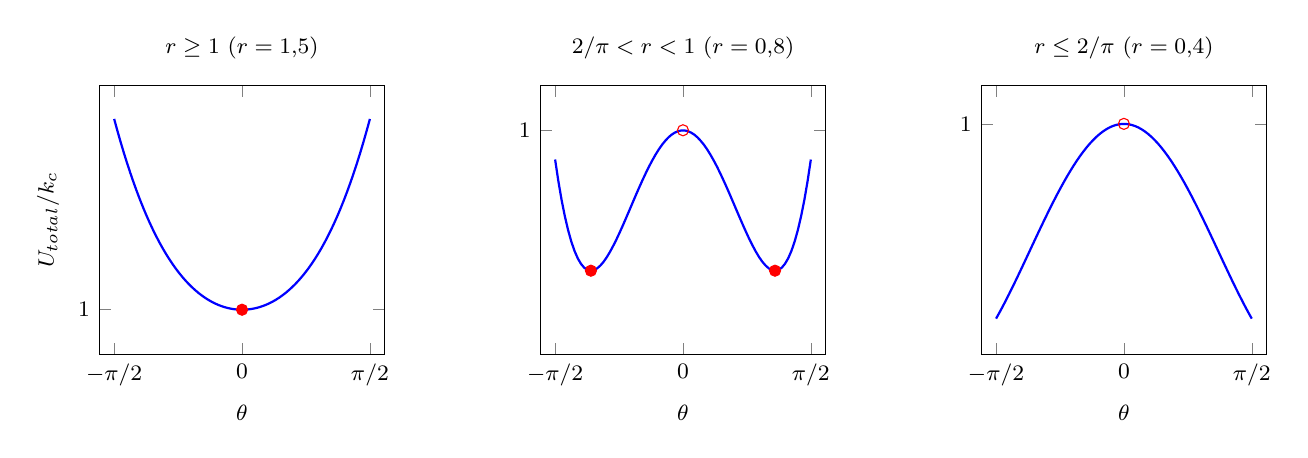
\begin{tikzpicture}
\begin{axis}[at={(0,0)}, width=5.2cm, height=5cm, domain=-1.5708:1.5708, samples=80, xmin=-1.75, xmax=1.75,
 xtick={-1.5708,0,1.5708}, xticklabels={$-\pi/2$,$0$,$\pi/2$}, xlabel={$\theta$}, ylabel={$U_{total}/k_c$},
 ymin=0.8, ymax=2.0, ytick={1}, title={\footnotesize $r\ge1$ ($r=1{,}5$)}, tick label style={font=\footnotesize}, label style={font=\footnotesize}]
\addplot[thick,blue]{cos(deg(x))+0.75*x^2};
\addplot[only marks,mark=*,red]coordinates{(0,1)};
\end{axis}
\begin{axis}[at={(5.6cm,0)}, width=5.2cm, height=5cm, domain=-1.5708:1.5708, samples=80, xmin=-1.75, xmax=1.75,
 xtick={-1.5708,0,1.5708}, xticklabels={$-\pi/2$,$0$,$\pi/2$}, xlabel={$\theta$},
 ymin=0.9, ymax=1.02, ytick={1}, title={\footnotesize $2/\pi<r<1$ ($r=0{,}8$)}, tick label style={font=\footnotesize}, label style={font=\footnotesize}]
\addplot[thick,blue]{cos(deg(x))+0.4*x^2};
\addplot[only marks,mark=*,red]coordinates{(1.131,0.9374)(-1.131,0.9374)};
\addplot[only marks,mark=o,red]coordinates{(0,1)};
\end{axis}
\begin{axis}[at={(11.2cm,0)}, width=5.2cm, height=5cm, domain=-1.5708:1.5708, samples=80, xmin=-1.75, xmax=1.75,
 xtick={-1.5708,0,1.5708}, xticklabels={$-\pi/2$,$0$,$\pi/2$}, xlabel={$\theta$},
 ymin=0.4, ymax=1.1, ytick={1}, title={\footnotesize $r\le2/\pi$ ($r=0{,}4$)}, tick label style={font=\footnotesize}, label style={font=\footnotesize}]
\addplot[thick,blue]{cos(deg(x))+0.2*x^2};
\addplot[only marks,mark=o,red]coordinates{(0,1)};
\end{axis}
\end{tikzpicture}
\end{center}

\noindent Resumo: $r\ge1$, poço simples em $\theta=0$; $2/\pi<r<1$, poço duplo (máximo local em $0$, mínimos em $\pm\theta_0$); $r\le2/\pi$, máximo único em $\theta=0$ e $U$ decrescente em $|\theta|$ (a haste tomba).

ANSWER: a) $k_c=MgL/2$. b) $k/k_c\ge1$: apenas $\theta=0$, estável; $2/\pi<k/k_c<1$: três equilíbrios, $\theta=0$ instável e $\pm\theta_0$ (com $\mathrm{sen}\,\theta_0/\theta_0=k/k_c$) estáveis; $0<k/k_c\le2/\pi$: apenas $\theta=0$, instável. c) $U_{total}=\frac{MgL}{2}\cos\theta+\frac12k\theta^2$: poço simples, poço duplo ou máximo único, respectivamente.%
\newpage%
\section*{Questão 2}

\section*{Solução}

\textbf{Hipóteses.} Resistência do ar desprezível; $g$ = aceleração da gravidade; $e=0{,}7$. Como o solo é perfeitamente liso, a força em cada choque é apenas normal (vertical). O impulso é, portanto, vertical, e $v_x$ \textbf{se conserva} ao longo de todo o movimento (também no voo, pois $a_x=0$). Na direção normal vale a definição do coeficiente de restituição: $|v_y'|=e\,|v_y|$ (afastamento $=e\cdot$ aproximação).

Condições iniciais:
\[
v_x=V\cos30^\circ=\frac{\sqrt3}{2}V,\qquad v_{y,0}=V\,\mathrm{sen}\,30^\circ=\frac V2 .
\]
Entre dois choques a energia mecânica se conserva. Logo a partícula retorna ao solo com $|v_y|$ igual ao de partida, e após o $k$-ésimo choque
\[
v_{y,k}=e^{k}\,\frac V2 .
\]

\textbf{a) Altura máxima após $n$ choques.} No voo que se segue ao $n$-ésimo choque, a altura máxima ocorre quando $v_y=0$. Por Torricelli (ou conservação de energia na vertical),
\[
H_n=\frac{v_{y,n}^2}{2g}=\frac{e^{2n}V^2}{8g}
=\frac{(0{,}49)^{n}\,V^2}{8g}.
\]
Verificação: $n=0$ dá $H_0=V^2\,\mathrm{sen}^2 30^\circ/(2g)=V^2/(8g)$, o resultado do lançamento oblíquo sem choque. Cada choque multiplica a altura por $e^2=0{,}49$.

\textbf{b) Tempo para a energia mínima.} Tomando o solo como referência de energia potencial, a energia mecânica é
\[
E=\underbrace{\tfrac12 m v_x^2}_{\text{constante}}+\underbrace{\tfrac12 m v_y^2+mgy}_{\text{parte vertical}} .
\]
Ela é constante entre choques e diminui em cada choque, pois só a componente vertical é afetada. Após $n$ choques (no início do voo, $y=0$):
\[
E_n=\frac38 mV^2+\frac18 mV^2e^{2n}.
\]
Para $n=0$ obtém-se $E_0=\tfrac12 mV^2$, como esperado. $E_n$ decresce monotonicamente e tende a
\[
E_{\min}=\tfrac12 m v_x^2=\frac38\,mV^2 ,
\]
que é atingida quando todo o movimento vertical se extingue. A massa passa então a deslizar sobre o solo com $v=\frac{\sqrt3}{2}V$.

O número de choques até esse ponto é infinito, mas o tempo total é finito. O voo $k$ ($k=0,1,2,\dots$) dura $\tau_k=2v_{y,k}/g=e^{k}V/g$. A soma é uma PG convergente ($e<1$):
\[
\Delta t=\sum_{k=0}^{\infty}\tau_k=\frac Vg\sum_{k=0}^{\infty}e^{k}=\frac{V}{g\,(1-e)}=\frac{V}{0{,}3\,g}=\frac{10\,V}{3\,g}\approx 3{,}3\,\frac Vg .
\]

\textbf{Conferência.} A unidade $V/g$ é de tempo. Para $e\to0$ resulta $\Delta t\to V/g$ (um único voo, e a massa fica colada ao solo). Para $e\to1$, $\Delta t\to\infty$ (sem perdas, a energia nunca diminui). Os dois limites são coerentes. A energia mínima é $\frac34$ da inicial, pois $E_{\min}/E_0=\frac{3/8}{1/2}$.

\medskip
\noindent Interpretamos ``energia'' como a energia mecânica total da massa. Seu mínimo só é atingido no limite em que os choques se acumulam, no instante $\Delta t$.

ANSWER: a) $H_n=\dfrac{(0{,}7)^{2n}V^2}{8g}=\dfrac{(0{,}49)^nV^2}{8g}$; b) $\Delta t=\dfrac{V}{g(1-e)}=\dfrac{10V}{3g}$%
\newpage%
\section*{Questão 3}

\section*{Solução}

\textbf{Hipóteses.} Sem resistência do ar; massa puntiforme, que parte do repouso em $(0,R,h)$ (borda do disco, sobre o eixo $y$); disco horizontal girando em torno de $z$ com $\omega=\alpha t$ (anti-horário visto de cima; o sentido não altera $d$ nem o tempo). O coeficiente $\mu_e$ vale entre massa e disco, e $\mu_c$ só entre massa e solo. Supomos $\mu_e g>\alpha R$; caso contrário a massa escorregaria já em $t=0$.

\subsection*{1) Permanência sobre o disco}
Sem aceleração vertical, $N=mg$. O atrito estático é a única força horizontal e deve fornecer a aceleração do ponto da borda, que tem componente tangencial $\alpha R$ e componente centrípeta $\omega^2R$, perpendiculares entre si:
\[
|\vec a_p|=R\sqrt{\alpha^2+\omega^4}\le \mu_e g .
\]
Como $|\vec a_p|$ cresce com $t$, o deslizamento começa no primeiro instante $t_1$ em que vale a igualdade:
\[
R^2\omega_1^4=\mu_e^2g^2-\alpha^2R^2
\;\Rightarrow\;
\omega_1^2R=Q^2,\qquad Q\equiv\left(\mu_e^2g^2-\alpha^2R^2\right)^{1/4}.
\]
Logo
\[
\omega_1=\frac{Q}{\sqrt R},\qquad t_1=\frac{\omega_1}{\alpha}=\frac{Q}{\alpha\sqrt R},\qquad v=\omega_1R=Q\sqrt R .
\]

\subsection*{2) Saída do disco}
Logo após $t_1$, o atrito (oposto ao deslizamento relativo, portanto paralelo a $\vec a_p$) não supre $m\vec a_p$. A aceleração relativa ao disco é $-(|\vec a_p|-f/m)\,\hat a_p$, e sua componente radial aponta para fora, pois $\omega_1^2R>0$. Como a massa já está na borda, ela deixa o disco sem percorrer distância apreciável, e sua velocidade de saída é a do ponto da borda: módulo $v$, horizontal e tangente à circunferência. Daí em diante só atua a gravidade (lançamento horizontal):
\[
t_q=\sqrt{\frac{2h}{g}},\qquad s=v\,t_q \ \text{(deslocamento horizontal, tangencial).}
\]

\subsection*{a) Distância do ponto de contato à origem}
Na saída, o ângulo percorrido a partir de $y$ é $\theta_1=\alpha t_1^2/2$. A posição é $(-R\,\mathrm{sen}\,\theta_1,\;R\cos\theta_1)$ e o versor tangente é $(-\cos\theta_1,-\mathrm{sen}\,\theta_1)$. O ponto de queda é
\[
(x_f,y_f)=\big(-R\,\mathrm{sen}\,\theta_1-s\cos\theta_1,\; R\cos\theta_1-s\,\mathrm{sen}\,\theta_1\big),
\]
e $x_f^2+y_f^2=R^2+s^2$ (raio e tangente são perpendiculares). Com $s^2=v^2\,\dfrac{2h}{g}=\dfrac{2hR}{g}\,Q^2$, resulta
\[
\boxed{d=\sqrt{R^2+\frac{2hR}{g}\sqrt{\mu_e^2g^2-\alpha^2R^2}}}
\]
O resultado independe de $\theta_1$ (em geral não é pequeno), então a aproximação $\mathrm{sen}\,\theta\approx\theta$ não é usada. Também independe do sentido de giro e de $\mu_c$.

\subsection*{b) Instante em que a massa para}
No contato com o solo, sem quicar, $v_z\to0$. Adotamos que a componente horizontal $v$ se conserva (impulso de atrito desprezado), conforme o enunciado: "realiza um deslizamento". A massa então desliza em linha reta, na direção da tangente, com $N=mg$ e atrito cinético constante $\mu_c mg$ oposto à velocidade. A desaceleração é $\mu_c g$, e
\[
t_d=\frac{v}{\mu_c g}=\frac{Q\sqrt R}{\mu_c g}.
\]
O instante de parada é a soma das três fases:
\[
\boxed{t_{\text{para}}=t_1+t_q+t_d=\sqrt{\frac{2h}{g}}+\sqrt R\,\big(\mu_e^2g^2-\alpha^2R^2\big)^{1/4}\left[\frac{1}{\alpha R}+\frac{1}{\mu_c g}\right]}
\]

\emph{Ressalva.} Se o atrito cinético atuasse de forma impulsiva durante o impacto, a velocidade horizontal seria $v'=v-\mu_c\sqrt{2gh}$ e teríamos $t_{\text{para}}=t_1+v/(\mu_c g)$, isto é, $\sqrt{2h/g}$ a menos. Se $v\le\mu_c\sqrt{2gh}$, a massa pararia no próprio choque. A parte (a) não muda.

\subsection*{Verificações}
\begin{itemize}
\item \emph{Unidades:} $Q^2$ é aceleração (m/s$^2$). $Q/(\alpha\sqrt R)$ e $Q\sqrt R/(\mu_c g)$ têm unidade de s. $\sqrt{2h/g}$ tem unidade de s. $d$ tem unidade de m.
\item \emph{Limite $\alpha R\to\mu_e g$:} $Q\to0$, então $d\to R$ e $t_{\text{para}}\to\sqrt{2h/g}$. A massa cai na vertical da borda e para ao tocar o solo.
\item \emph{Limite $\alpha\to0$:} $v\to\sqrt{\mu_e gR}$, a velocidade máxima de uma curva com atrito. Quando $\mu_c\to0$, $t_d\to\infty$: a massa desliza sem parar, como esperado.
\item \emph{Exemplo numérico} ($g=9,8$ m/s$^2$; $\mu_e=0,5$; $\mu_c=0,3$; $R=2$ m; $\alpha=0,5$ rad/s$^2$; $h=1,2$ m): $Q^2=4,797$ m/s$^2$; $\omega_1=1,549$ rad/s; $t_1=3,097$ s; $v=3,097$ m/s. O critério de atrito é satisfeito: $R\sqrt{\alpha^2+\omega_1^4}=4,90=\mu_e g$. Em seguida, $t_q=0,495$ s; $s=1,533$ m; $\theta_1=2,398$ rad; $(x_f,y_f)=(-0,225;\,-2,510)$ m; $d=2,520$ m, que coincide com $\sqrt{x_f^2+y_f^2}$. Por fim, $t_d=1,054$ s e $t_{\text{para}}=4,646$ s.
\end{itemize}

ANSWER: a) $d=\sqrt{R^{2}+\dfrac{2hR}{g}\sqrt{\mu_e^{2}g^{2}-\alpha^{2}R^{2}}}$; b) $t_{\text{para}}=\sqrt{\dfrac{2h}{g}}+\sqrt{R}\,\big(\mu_e^{2}g^{2}-\alpha^{2}R^{2}\big)^{1/4}\left[\dfrac{1}{\alpha R}+\dfrac{1}{\mu_c g}\right]$%
\newpage%
\section*{Questão 4}

\section*{Solução}

\textbf{Dados e estado inicial.} Com vácuo acima do pistão e o recipiente de massa desprezível, a única força para baixo sobre o pistão é o peso de $m+M$. No equilíbrio inicial,
\[
P_iA=(m+M)g,\qquad V_i=Ah_i .
\]
Sem a areia, o equilíbrio exige $P_fA=mg$. Para o gás monoatômico, $U=\tfrac32 nRT=\tfrac32 PV$ e $\gamma=c_p/c_v=\tfrac53$.

\medskip
\textbf{a) Retirada lenta (quase estática).}

As paredes e o pistão são adiabáticos, logo $Q=0$. A retirada grão a grão mantém o gás em equilíbrio a cada instante e sem dissipação. O processo é, portanto, adiabático reversível:
\[
PV^{\gamma}=\text{cte}\;\Rightarrow\;P_i\,(Ah_i)^{5/3}=P_f\,(Ah_f)^{5/3}.
\]
Com $P_i/P_f=(m+M)/m$:
\[
\boxed{h_f=h_i\left(\frac{m+M}{m}\right)^{3/5}=h_i\left(1+\frac{M}{m}\right)^{3/5}}
\]
Verificação: para $M=0$ obtém-se $h_f=h_i$. Para $M>0$, $h_f>h_i$, pois o gás expande ao diminuir a carga.

\medskip
\textbf{b) Retirada instantânea.}

Logo após a retirada, o gás ainda está a $P_i$, mas o pistão pesa só $mg$. A força resultante para cima é $Mg$, e o pistão sobe acelerado. Ele ultrapassa a posição de equilíbrio $h_f$ e para momentaneamente em $h_{max}$, onde $v=0$. Neste ponto a pressão do gás \emph{não} é $mg/A$, pois o pistão está sendo freado, com aceleração para baixo.

\emph{Hipóteses.} Não há atrito nem vácuo a dissipar energia. O pistão é muito mais lento que as moléculas, então o gás tem $P$ e $T$ uniformes a cada instante. Sem dissipação no gás, a evolução após o desequilíbrio inicial é adiabática reversível, com $PV^{5/3}=\text{cte}$. Isso fixa o estado do gás em $h_{max}$:
\[
P_{max}=P_i\left(\frac{h_i}{h_{max}}\right)^{5/3}.
\]

\emph{Energia.} Tomando gás e pistão como sistema, com $Q=0$ e nada acima do pistão, a energia interna do gás converte-se em energia potencial do pistão. Em $h_{max}$ a energia cinética é nula:
\[
\Delta U+mg\,(h_{max}-h_i)=0 .
\]
Com $U=\tfrac32PV$:
\[
\tfrac32\left(P_iAh_i-P_{max}Ah_{max}\right)=mg\,(h_{max}-h_i).
\]
Substituindo $P_iA=(m+M)g$ e $P_{max}$, e simplificando $g$:
\[
\tfrac32 (m+M)h_i\left[1-\left(\frac{h_i}{h_{max}}\right)^{2/3}\right]=m\,(h_{max}-h_i),
\]
ou seja,
\[
\boxed{\,3\,(m+M)\,h_i\left[1-\left(\frac{h_i}{h_{max}}\right)^{2/3}\right]=2\,m\,(h_{max}-h_i)\,}
\]

A raiz $h_{max}=h_i$ é trivial (instante inicial, $v=0$); a solução procurada é a raiz $h_{max}>h_i$. Com $y=(h_{max}/h_i)^{1/3}$, e cancelando o fator $(y-1)$, a equação vira o polinômio
\[
2m\,y^4+2m\,y^3+2m\,y^2-3\,(m+M)\,y-3\,(m+M)=0 .
\]

\textbf{Verificações.}
\begin{itemize}
\item $M\to0$: $h_{max}\to h_i$. Sem desequilíbrio, o pistão não se move.
\item $M\ll m$: com $h_{max}=h_i(1+\varepsilon)$, a expansão a segunda ordem dá $\varepsilon\approx \dfrac{6M}{5m}$. Isso é o dobro do deslocamento até o equilíbrio, $h_f/h_i-1\approx \dfrac{3M}{5m}$, como num oscilador quase harmônico que parte do repouso.
\item $M\gg m$: $h_{max}\approx \dfrac{3(m+M)}{2m}\,h_i$, ou seja, $\tfrac32P_iV_i\approx mg\,\Delta h$. O gás cede quase toda a sua energia interna ao pistão.
\item $h_{max}>h_f$ sempre (por exemplo, $m=M$: $h_f\approx1,52\,h_i$ e $h_{max}\approx2,26\,h_i$). O pistão oscila entre $h_i$ e $h_{max}$ em torno de $h_f$. A conferência numérica, integrando a equação de movimento do pistão, reproduz esses valores.
\item Unidades: todos os termos da equação têm dimensão de comprimento, e $(m+M)/m$ é adimensional.
\end{itemize}

\medskip
ANSWER: a) $h_f=h_i\,(1+M/m)^{3/5}$; \quad b) $3(m+M)\,h_i\left[1-(h_i/h_{max})^{2/3}\right]=2m\,(h_{max}-h_i)$, com $h_{max}>h_i$.%
\newpage%
\section*{Questão 5}

\section*{Solução}

\textbf{Convenções e hipóteses.} Luz se propaga da esquerda para a direita, com o vértice $V$ na origem e o eixo de simetria como eixo $x$. O centro de curvatura $C$ está em $x=-R$ (do lado de $n_1$) e as fontes em $x=-p$, a alturas $\pm h$. Vale a aproximação paraxial (ângulos pequenos, $\mathrm{sen}\,\theta\approx\theta\approx\mathrm{tg}\,\theta$), e $\lambda\ll p$ garante a validade da óptica geométrica.

\subsection*{a) Posição da imagem}

\textbf{Posição horizontal $p'$.} Tome uma fonte sobre o eixo. Um raio sai dela e atinge a interface a uma altura $y$ pequena.
\begin{itemize}
\item Inclinação do raio incidente: $\alpha_1=y/p$.
\item A normal nesse ponto passa por $C$, logo sua inclinação é $\varphi=y/R$.
\item Ângulo de incidência: $\theta_1=\alpha_1-\varphi=y\left(\dfrac1p-\dfrac1R\right)$.
\item Lei de Snell paraxial: $n_1\theta_1=n_2\theta_2$, logo $\theta_2=\dfrac{n_1}{n_2}\theta_1$.
\item Inclinação do raio refratado: $\alpha_2=\varphi+\theta_2$, ou seja,
\[
\frac{\alpha_2}{y}=\frac1R+\frac{n_1}{n_2}\left(\frac1p-\frac1R\right)=\frac{n_1}{n_2p}+\frac{n_2-n_1}{n_2R}>0 .
\]
\end{itemize}
O raio refratado sobe com inclinação $\alpha_2$ a partir da altura $y$. Ele cruza o eixo em $x=-y/\alpha_2$, e esse é o ponto $p'$ (o resultado independe de $y$, logo há formação de imagem). Assim $n_2/p'=-n_1/p-(n_2-n_1)/R$, ou seja,
\[
\frac{n_1}{p}+\frac{n_2}{p'}=-\frac{n_2-n_1}{R}
\qquad\Longrightarrow\qquad
\boxed{\,p'=-\,\frac{n_2\,R\,p}{n_1R+(n_2-n_1)\,p}\,}
\]
Como $n_2>n_1$, o denominador é positivo e $p'<0$. A imagem é \emph{virtual}, fica no lado de $n_1$ (à esquerda do vértice), a uma distância $|p'|=\dfrac{n_2Rp}{n_1R+(n_2-n_1)p}$ da interface.

\textbf{Posições verticais.} Considere o raio da fonte superior (altura $h$) que incide no vértice, onde a normal é o próprio eixo.
\begin{itemize}
\item Incidência: $\theta_1=h/p$.
\item Refração: $n_1\theta_1=n_2\theta_2$, logo $\theta_2=\dfrac{n_1h}{n_2p}$. O raio desce com essa inclinação.
\item O prolongamento para trás desse raio, em $x=p'$, está à altura $h'=\theta_2\,|p'|$.
\end{itemize}
Substituindo $|p'|$:
\[
\boxed{\,y'_{\pm}=\pm\,h'=\pm\,\frac{n_1\,R\,h}{n_1R+(n_2-n_1)\,p}\,}
\]
Equivalentemente, a ampliação é $m=-\dfrac{n_1p'}{n_2p}=\dfrac{n_1R}{n_1R+(n_2-n_1)p}$, com $0<m\le1$. As imagens são direitas, menores que os objetos, e ficam no mesmo semiplano de cada fonte.

\emph{Conferências.} Para $n_2=n_1$ obtém-se $p'=-p$ e $h'=h$. Para $p\to0$, $h'=h$. Para $p\to\infty$, $p'\to-n_2R/(n_2-n_1)$, que é o foco virtual de uma superfície divergente. Um traçado numérico exato de raios (com $n_1=1$, $n_2=1,5$, $R=10$, $p=5$) deu $p'=-6,0000$ e $h'/h=0,8000$, em acordo com as fórmulas.

\subsection*{b) Interferência para $R\to\infty$}

Com $R\to\infty$ a interface é plana. De (a), $p'=-\dfrac{n_2}{n_1}p$ e $h'=h$. Os raios que entram em $n_2$ parecem vir de duas fontes virtuais coerentes, em fase, em $y=\pm h$. Elas estão a $n_2p/n_1$ à esquerda da interface, separadas por $d=2h$.

A distância dessas fontes à tela é $L=D+\dfrac{n_2}{n_1}p\approx D$, pois $p\ll D$.

A frequência não muda na refração. Tomando $\lambda$ como o comprimento de onda no meio $n_1$ (onde estão as fontes), em $n_2$ tem-se $\lambda_2=\dfrac{n_1}{n_2}\lambda$.

Para um ponto da tela à altura $y$, com $y,h\ll L$, a diferença de percurso é
\[
\delta=\sqrt{L^2+(y+h)^2}-\sqrt{L^2+(y-h)^2}\approx\frac{2hy}{L}\approx\frac{2hy}{D}.
\]
Em $y=0$ tem-se $\delta=0$, que é o máximo central (ponto luminoso central). A primeira franja luminosa ocorre em $\delta=\lambda_2$:
\[
\frac{2h\,y_1}{D}=\frac{n_1}{n_2}\lambda
\qquad\Longrightarrow\qquad
\boxed{\,y_1=\frac{n_1}{n_2}\,\frac{\lambda D}{2h}\,}
\]

\emph{Verificação independente.} Pelo princípio de Fermat, o caminho óptico de uma fonte a $h$ até $y$ na tela, passando pela interface plana, é $n_1p+n_2D+\dfrac{n_1n_2(y-h)^2}{2(n_1D+n_2p)}$. Isso equivale a uma fonte em $n_2$ a distância $L$, como usado acima.

\emph{Observações.}
\begin{itemize}
\item Dimensionalmente, $y_1$ é um comprimento.
\item Para $n_2=n_1$, recupera-se o resultado de Young, $\lambda D/(2h)$.
\item A franja se afasta menos do centro em $n_2>n_1$, pois $\lambda_2<\lambda$.
\item Se $\lambda$ fosse o comprimento de onda no vácuo, bastaria trocar $n_1\lambda$ por $\lambda$, obtendo $y_1=\lambda D/(2n_2h)$.
\end{itemize}

ANSWER: (a) $p'=-\dfrac{n_2Rp}{n_1R+(n_2-n_1)p}$ (imagem virtual, no lado de $n_1$); imagens em $y'=\pm\dfrac{n_1Rh}{n_1R+(n_2-n_1)p}$. (b) $y_1=\dfrac{n_1\lambda D}{2n_2h}$.%
\newpage%
\section*{Questão 6}

\section*{Solução}

\textbf{Hipóteses.} Voltímetro e fios ideais; $d\ll a$, logo as placas formam um capacitor plano ideal: $C=\varepsilon_0A/d$ na situação inicial e $C'=\varepsilon_0A/d'$ para separação $d'$. No equilíbrio ($t_3$) não há corrente, então o capacitor e as placas têm a mesma diferença de potencial $V_3$, lida no voltímetro. O efeito pendular (componente horizontal do peso, onde entraria $\mathrm{sen}\,\theta\approx\theta$) é \emph{desprezado}, pois o enunciado não dá massas nem comprimento dos fios. Assim, na horizontal só atuam a força elétrica e a força da mola.

\textbf{Leitura do dado.} Em $t_2$ o capacitor está carregado, com tensão $\varepsilon$ (é o que o voltímetro marca nesse instante). Logo $V_3=\varepsilon/4$. (O valor $\varepsilon/2$ é a tensão logo após fechar $S_2$ com $d$ ainda fixo, e não a de $t_2$. A leitura alternativa $V_3=\varepsilon/8$ é descartada no final.)

\textbf{a) Carga que fluiu.} Com $S_1$ aberta, o conjunto \{placa superior do capacitor, fio, placa 1\} está isolado, assim como o conjunto \{placa inferior do capacitor, fio, placa 2\}. Conservação da carga em cada um, com $Q_0=C\varepsilon$ e as placas inicialmente neutras:
\[
C\varepsilon=CV_3+q_1,\qquad -C\varepsilon=-CV_3+q_2 .
\]
Portanto $q_1=-q_2=q=C(\varepsilon-V_3)$, ou seja,
\[
\boxed{q=\frac{3}{4}\,C\varepsilon}.
\]

\textbf{b) Deformação da mola.} As placas têm carga $\pm q$ e tensão $V_3$:
\[
C'=\frac{q}{V_3}=\frac{3C\varepsilon/4}{\varepsilon/4}=3C
\;\Rightarrow\; \frac{\varepsilon_0A}{d'}=3\,\frac{\varepsilon_0A}{d}\;\Rightarrow\; d'=\frac d3 .
\]
A atração elétrica aproxima as placas, e a mola é \emph{comprimida}:
\[
\boxed{x=d-d'=\frac{2d}{3}}\quad(\text{compressão}).
\]

\textbf{c) Constante elástica.} O campo de uma placa (grande, $d'\ll a$) é $E_1=\sigma/2\varepsilon_0=q/(2\varepsilon_0A)$, e a força sobre a outra placa é
\[
F_e=qE_1=\frac{q^2}{2\varepsilon_0A}=\frac{(3C\varepsilon/4)^2}{2Cd}=\frac{9\,C\varepsilon^2}{32\,d},
\]
usando $\varepsilon_0A=Cd$. Conferência independente: $F_e=\dfrac{\varepsilon_0AV_3^2}{2d'^2}=\dfrac12\,Cd\,\dfrac{\varepsilon^2}{16}\,\dfrac{9}{d^2}$, que dá o mesmo valor.

No equilíbrio, a força da mola em cada placa iguala a força elétrica, $kx=F_e$:
\[
k=\frac{F_e}{x}=\frac{9C\varepsilon^2}{32\,d}\cdot\frac{3}{2d}=\boxed{\frac{27\,C\,\varepsilon^2}{64\,d^2}=\frac{27\,\varepsilon_0\,a^2\,\varepsilon^2}{64\,d^3}}.
\]

\textbf{Conferências.}
\begin{itemize}
\item \emph{Unidades:} $C\varepsilon^2$ é energia (J), então $C\varepsilon^2/d^2$ está em J/m$^2$ = N/m. Além disso, $q<Q_0$ e $d'<d$, como esperado.
\item \emph{Balanço de energia} (em unidades de $C\varepsilon^2$). Inicial: $\tfrac12=\tfrac{16}{32}$. Final: capacitor $\tfrac12CV_3^2=\tfrac1{32}$; placas $\tfrac{q^2}{2C'}=\tfrac{3}{32}$; mola $\tfrac12kx^2=\tfrac{3}{32}$, total $\tfrac{7}{32}$. Foram dissipados $\tfrac{9}{32}C\varepsilon^2>0$ (efeito Joule nos fios e amortecimento mecânico). Por isso a energia \emph{não} se conserva, e o método correto é conservação de carga mais equilíbrio de forças. O sinal positivo da dissipação é consistente.
\item \emph{Estabilidade e a leitura do dado.} Para separação $s$ qualquer, a carga conservada dá $V=\varepsilon s/(s+d)$. A força líquida sobre uma placa, no sentido de aumentar $s$, é
\[
F_{\text{liq}}(s)=k(d-s)-\frac{Cd\,\varepsilon^2}{2(s+d)^2}.
\]
Com o $k$ obtido, esta força se fatora como $F_{\text{liq}}=-\dfrac{C\varepsilon^2(3s-d)^2(3s+5d)}{64\,d^2(s+d)^2}\le0$. Ela se anula, com raiz dupla, em $s=d/3$. Logo esse equilíbrio é o limite de estabilidade (semiestável: estável pelo lado $s>d/3$ e instável pelo lado $s<d/3$). Em geral, um equilíbrio estável exige $s>d/3$, isto é, $V_3>\varepsilon/4$. A leitura $V_3=\varepsilon/8$ levaria a $s=d/7<d/3$, equilíbrio instável, e por isso foi descartada.
\item Chegar a $s=d/3$ partindo de $s=d$ exige dissipação forte (aproximação assintótica, sobreamortecida). Com pouca dissipação, as placas ultrapassam $d/3$ e colapsam. Isso é uma idealização do enunciado e não altera os itens pedidos.
\end{itemize}

ANSWER: a) $q=\dfrac{3}{4}C\varepsilon$; b) compressão $x=\dfrac{2d}{3}$ (distância final $d/3$); c) $k=\dfrac{27\,C\,\varepsilon^{2}}{64\,d^{2}}=\dfrac{27\,\varepsilon_0 a^2\varepsilon^2}{64\,d^3}$%
\newpage%
\section*{Questão 7}

\section*{Solução}

\textbf{Modelo.} O voltímetro é ideal (resistência infinita), logo não há corrente no ramo $DB$. Assim $R_1$ e $R_3$ estão em série entre $A$ e $C$, e $R_2$ e $R_4$ também. Pela figura, o terminal positivo da fonte (placa maior) está em $A$, então $V_A=V_s$ e $V_C=0$. Se a polaridade fosse a oposta, só o sinal de $V_o$ mudaria, e não o módulo nem as conclusões. Cada ramo é um divisor de tensão:
\[
V_D=V_s\,\frac{R_3}{R_1+R_3},\qquad V_B=V_s\,\frac{R_4}{R_2+R_4}.
\]

\textbf{Linearização.} Escrevo $R_i=R_0(1+x_i)$ com $|x_i|\ll 1$. Para resistor constante, $x_i=0$. Para extensômetro, $x_i=G\varepsilon_i+\alpha\Delta T$. Usando $(1+x)^{-1}\approx 1-x$ e desprezando produtos de pequenas quantidades:
\[
V_D=\frac{V_s}{2}\,(1+x_3)\Big[1+\frac{x_1+x_3}{2}\Big]^{-1}\approx\frac{V_s}{2}\,(1+x_3)\Big[1-\frac{x_1+x_3}{2}\Big]\approx\frac{V_s}{2}\Big[1+\frac{x_3-x_1}{2}\Big],
\]
e, analogamente, $V_B\approx\dfrac{V_s}{2}\Big[1+\dfrac{x_4-x_2}{2}\Big]$. Portanto
\[
\boxed{V_o=V_D-V_B\approx\frac{V_s}{4}\,\big(x_2+x_3-x_1-x_4\big)}
\]
Com $x_i=0$ para todo $i$ obtém-se $V_o=0$ (ponte equilibrada), como esperado.

\textbf{a)} Seja o extensômetro em $R_1$ e $R_2=R_3=R_4=R_0$, com $x=G\varepsilon+\alpha\Delta T$. Então $V_B=V_s/2$ e
\[
V_D=\frac{V_s}{2+x}=\frac{V_s}{2}\Big(1+\frac{x}{2}\Big)^{-1}\approx\frac{V_s}{2}\Big(1-\frac{x}{2}\Big)
\;\Rightarrow\; V_o=V_D-V_B\approx-\frac{V_s}{4}\,x .
\]
(O resultado exato é $V_o=-V_s\,x/[2(2+x)]$.) Se o extensômetro estivesse em $R_3$, resultaria $V_o=+V_s x/4$. Em $R_2$ o sinal é $+$ e em $R_4$ é $-$, o que também decorre da fórmula geral. Em qualquer braço o módulo é o mesmo:
\[
|V_o|=\frac{V_s}{4}\,\big|G\varepsilon+\alpha\Delta T\big|.
\]
Ordem de grandeza: para $G\approx2$ e $\varepsilon=10^{-3}$, $x=2\cdot10^{-3}$. O valor linear é $5\cdot10^{-4}\,V_s$ e o exato é $4{,}995\cdot10^{-4}\,V_s$, com erro relativo $x/2=10^{-3}$, coerente com o regime linear.

Observação: a temperatura entra exatamente como a deformação, então um único extensômetro não separa $\varepsilon$ de $\Delta T$. Esse problema é resolvido no item b).

\textbf{b)} Seja $s_i=+1$ (extensômetro em ponto de tração), $-1$ (extensômetro em ponto de compressão) ou $0$ (resistor $R_0$). Como $|\varepsilon_i|=|\varepsilon|$ e $\Delta T$ é o mesmo para todos, $x_i=s_i G\varepsilon+|s_i|\,\alpha\Delta T$. Substituindo em $V_o$:
\[
V_o=\frac{V_s}{4}\Big[G\varepsilon\,\underbrace{(s_2+s_3-s_1-s_4)}_{\text{sensibilidade a }\varepsilon}+\alpha\Delta T\,\underbrace{(|s_2|+|s_3|-|s_1|-|s_4|)}_{\text{sensibilidade a }\Delta T}\Big].
\]
Há dois critérios de projeto.
\begin{itemize}
\item \emph{Compensação térmica:} $|s_2|+|s_3|=|s_1|+|s_4|$, isto é, o número de extensômetros nos braços $R_2,R_3$ deve ser igual ao número nos braços $R_1,R_4$. Um extensômetro ao lado de um $R_0$ fixo não compensa $\Delta T$. Por exemplo, $R_2$ e $R_3$ extensômetros com $R_1=R_4=R_0$ dão $V_o=\tfrac{V_s}{2}(G\varepsilon+\alpha\Delta T)$, em que $\Delta T$ soma e não se distingue de $\varepsilon$.
\item \emph{Sensibilidade máxima a $\varepsilon$:} como $|s_i|\le1$, vale $|s_2+s_3-s_1-s_4|\le4$. A igualdade exige $s_2=s_3=-s_1=-s_4=\pm1$. Então os quatro dispositivos são extensômetros, e esse caso já satisfaz a compensação térmica.
\end{itemize}
Entre as montagens compensadas, a meia ponte (dois extensômetros em braços adjacentes, em pontos de tipos opostos, os outros dois $R_0$) dá $|V_o|=V_sG|\varepsilon|/2$. A ponte completa dá o dobro disso. Uma varredura numérica das $3^4$ combinações, restrita às compensadas termicamente, confirma esse máximo.

\textbf{Montagem.} Os quatro dispositivos são extensômetros, sem nenhum $R_0$:
\begin{itemize}
\item $R_2$ e $R_3$ (braços opostos) em pontos de \textbf{tração};
\item $R_1$ e $R_4$ (braços opostos) em pontos de \textbf{compressão}.
\end{itemize}
Os braços adjacentes ficam sempre em tipos diferentes. A montagem espelhada ($R_1,R_4$ em tração e $R_2,R_3$ em compressão) é equivalente e só inverte o sinal de $V_o$. Então $x_2=x_3=G\varepsilon+\alpha\Delta T$ e $x_1=x_4=-G\varepsilon+\alpha\Delta T$, o que dá
\[
V_o=\frac{V_s}{4}\,4G\varepsilon=V_s\,G\,\varepsilon .
\]
Isso é quatro vezes o sinal do item a), e a parcela $\alpha\Delta T$ se cancela. Sem aproximação, os divisores dão $V_o=V_sG\varepsilon/(1+\alpha\Delta T)\approx V_sG\varepsilon(1-\alpha\Delta T)$. O resíduo é do tipo $\varepsilon\alpha\Delta T$, desprezível pelo enunciado. Ele só altera levemente o ganho e não cria um sinal de deslocamento (\emph{offset}) térmico.

ANSWER: a) $|V_o|=\dfrac{V_s}{4}\,|G\varepsilon+\alpha\Delta T|$. b) Os quatro dispositivos devem ser extensômetros, sem $R_0$ fixo: $R_2$ e $R_3$ em pontos de tração e $R_1$ e $R_4$ em pontos de compressão (ou o inverso). Isso dá $|V_o|=V_sG|\varepsilon|$, sem efeito de $\Delta T$ em primeira ordem.%
\newpage%
\section*{Questão 8}

\section*{Solução}

\textbf{Convenções.} Seja $\hat{x}$ o sentido de $\vec B$ (da esquerda para a direita, ao longo da linha de campo que contém os pontos 1 e 2). Decompomos $\vec v$ em
\[
v_\parallel = v\cos\theta \quad (\text{paralela a } \vec B), \qquad v_\perp = v\,\mathrm{sen}\,\theta \quad (\text{perpendicular a } \vec B).
\]

\subsection*{a) Módulo da velocidade ao entrar na região de campo}

Entre o repouso e a entrada na região magnética só atua a força elétrica (conservativa), no vácuo. Pelo teorema trabalho--energia cinética, com velocidades não relativísticas:
\[
qV=\frac{1}{2}mv^{2}
\quad\Longrightarrow\quad
\boxed{v=\sqrt{\frac{2qV}{m}}}
\]

\subsection*{b) Tipo de movimento}

Na região, a única força é a magnética, $\vec F=q\vec v\times\vec B$. Ela é perpendicular a $\vec B$ e a $\vec v$. Isso implica:

\begin{itemize}
\item \textbf{Direção de $\vec B$:} $F_\parallel=0$. Logo $v_\parallel=v\cos\theta$ é \emph{constante}, e o movimento nessa direção é retilíneo uniforme.
\item \textbf{Plano perpendicular a $\vec B$:} como $\vec F\perp\vec v$, a força não realiza trabalho e $|\vec v|$ é constante. Portanto $v_\perp=v\,\mathrm{sen}\,\theta$ também é constante. A força, de módulo constante $qv_\perp B$, é sempre perpendicular a $\vec v_\perp$ e está nesse plano. A projeção do movimento nesse plano é, então, um \emph{movimento circular uniforme} de raio e período
\[
R=\frac{mv_\perp}{qB}=\frac{mv\,\mathrm{sen}\,\theta}{qB},
\qquad
T=\frac{2\pi R}{v_\perp}=\frac{2\pi m}{qB}.
\]
O período não depende de $v$ nem de $\theta$.
\end{itemize}

Superpondo um movimento retilíneo uniforme ao longo de $\vec B$ e um circular uniforme no plano perpendicular (com $v_\parallel\neq0$ e $v_\perp\neq0$, pois $0<\theta<90^\circ$ na figura), a trajetória é uma \textbf{hélice circular} de raio $R$ e passo constante $p=v_\parallel T$. O movimento é \textbf{helicoidal uniforme}, com $|\vec v|$ constante.

\subsection*{c) Condição sobre $\cos\theta$ para passar pelo ponto 2}

A linha de campo que passa por 1 projeta-se, no plano perpendicular a $\vec B$, em um único ponto. Esse ponto pertence à circunferência descrita pela projeção, pois a partícula parte dele. A partícula só volta a essa linha quando completa voltas inteiras:
\[
t_n=nT,\qquad n=1,2,3,\dots
\]
Em cada retorno, o deslocamento ao longo de $\vec B$ é
\[
x_n=v_\parallel t_n=n\,(v\cos\theta)\,\frac{2\pi m}{qB}=n\,p .
\]
Para passar pelo ponto 2 é preciso $x_n=L$ para algum $n$ inteiro positivo:
\[
L=n\,\frac{2\pi m\,v\cos\theta}{qB}
\quad\Longrightarrow\quad
\cos\theta=\frac{qBL}{2\pi n\,m\,v}.
\]
Substituindo $v=\sqrt{2qV/m}$, temos $\dfrac{q}{m\,v}=\sqrt{\dfrac{q}{2mV}}$, logo
\[
\boxed{\cos\theta=\frac{LB}{2\pi n}\sqrt{\frac{q}{2mV}},\qquad n=1,2,3,\dots}
\]

\textbf{Validade e conferências.}
\begin{itemize}
\item Como $0<\cos\theta<1$, os valores admissíveis de $n$ satisfazem $n>\dfrac{LB}{2\pi}\sqrt{\dfrac{q}{2mV}}$. O caso limite $\cos\theta\to1$ ($\theta\to0$) é a partícula descendo reta pela linha de campo, sem hélice.
\item Dimensões: $[qB/m]=\mathrm{s^{-1}}$ e $[L/v]=\mathrm{s}$, então $\cos\theta$ é adimensional. O fator $\sqrt{q/(2mV)}\,B$ tem dimensão de $\mathrm{m^{-1}}$, que se cancela com $L$.
\item Para cada $n$ permitido há um $\theta$ distinto. Os retornos seguintes ($n$ maiores) correspondem a ângulos maiores, isto é, a passos menores $p=L/n$.
\end{itemize}

ANSWER: a) $v=\sqrt{2qV/m}$; b) movimento helicoidal uniforme (MRU ao longo de $\vec B$ com $v\cos\theta$, MCU no plano perpendicular com $R=mv\,\mathrm{sen}\,\theta/(qB)$ e $T=2\pi m/(qB)$); c) $\cos\theta=\dfrac{LB}{2\pi n}\sqrt{\dfrac{q}{2mV}}$, com $n=1,2,3,\dots$ (e $\cos\theta<1$).%
\newpage%
\section*{Questão 9}

\section*{Solução}

\textbf{Hipóteses.} Vácuo, ondas planas, linearmente polarizadas em $\hat z$, de mesma amplitude $E_0$ e coerentes; $kd=n\pi$, com $n=0,1,2,\dots$

\subsection*{a) Reescrevendo $\vec E$}

Como $k(x+d)=kx+n\pi$, usamos $\cos(\theta+n\pi)=(-1)^n\cos\theta$ com $\theta=kx-\omega t$:
\[
\vec E=E_0\left[\cos(kx-\omega t+n\pi)+\cos(kx-\omega t)\right]\hat z
=E_0\left[1+(-1)^n\right]\cos(kx-\omega t)\,\hat z .
\]

(Pela identidade de soma de cossenos, o resultado equivalente é $\vec E=2E_0\cos\frac{n\pi}{2}\cos\!\left(kx-\omega t+\frac{n\pi}{2}\right)\hat z$, que coincide com o acima para todo $n$ inteiro.)

A fase $kx-\omega t$ é constante em $x=(\omega/k)\,t+\text{const.}$ Logo, a velocidade de fase é $\omega/k=c>0$ e a onda se propaga no sentido $x>0$. Sua amplitude depende apenas de $E_0$ e $n$:
\[
\boxed{E_{\text{res}}=E_0\left[1+(-1)^n\right]=\begin{cases}2E_0,& n\ \text{par}\\[2pt] 0,& n\ \text{ímpar}\end{cases}}
\]

\subsection*{b) Tipo de interferência}

Como $k=2\pi/\lambda$, a condição $kd=n\pi$ equivale a $d=n\lambda/2$.

\begin{itemize}
\item $n$ \textbf{par} ($d=0,\lambda,2\lambda,\dots$): as ondas estão em fase. A interferência é \textbf{construtiva total}, com amplitude $2E_0$ e intensidade $4$ vezes a de uma onda isolada ($I\propto E^2$).
\item $n$ \textbf{ímpar} ($d=\lambda/2,3\lambda/2,\dots$): as ondas estão em oposição de fase. A interferência é \textbf{destrutiva total}, e o campo resultante é nulo em todo ponto e instante.
\end{itemize}

\subsection*{c) Campo magnético}

Seja $E_z(x,t)=E_m\cos(kx-\omega t)$, com $E_m=E_0[1+(-1)^n]$. Como $\vec E$ só tem componente $z$ e depende só de $x$ e $t$, a lei de Faraday, $\nabla\times\vec E=-\partial\vec B/\partial t$, dá
\[
(\nabla\times\vec E)_y=-\frac{\partial E_z}{\partial x}
\;\Rightarrow\;
\frac{\partial B_y}{\partial t}=\frac{\partial E_z}{\partial x}=-kE_m\,\mathrm{sen}(kx-\omega t),
\]
e as demais componentes de $\vec B$ são nulas. Integrando em $t$ (sem campo estático):
\[
B_y=-\frac{k}{\omega}E_m\cos(kx-\omega t)=-\frac{E_m}{c}\cos(kx-\omega t),
\qquad \frac{\omega}{k}=c .
\]

Portanto $\vec B$ é perpendicular a $\vec E$ e à direção de propagação, e está em fase com $\vec E$. Ele aponta no sentido de $-\hat y$ quando $E_z>0$, de modo que $\vec E\times\vec B$ aponta em $+\hat x$ (verificação: $\hat z\times(-\hat y)=+\hat x$).

A amplitude do campo magnético resultante é $B_0=E_m/c=2E_0/c$ para $n$ par. Então
\[
\boxed{\vec B=-B_0\cos(kx-\omega t)\,\hat y,\qquad B_0=\frac{2E_0}{c}\quad(n\ \text{par})}
\]

Para $n$ ímpar, $E_m=0$ e, portanto, $\vec B=\vec 0$ (isto é, $B_0=0$). De forma geral, $\vec B=-\dfrac{E_0}{c}\left[1+(-1)^n\right]\cos(kx-\omega t)\,\hat y$. Se $B_0$ designasse a amplitude de cada onda componente ($E_0/c$), teríamos $\vec B=-B_0[1+(-1)^n]\cos(kx-\omega t)\,\hat y$.

\textbf{Conferência.} $n=0$ ($d=0$): as ondas coincidem e $\vec E=2E_0\cos(kx-\omega t)\hat z$, como em (a). $n=1$: $\cos(\theta+\pi)+\cos\theta=0$. As unidades estão corretas: $E_0/c$ tem unidade de campo magnético (T), e $|\vec E|/|\vec B|=c$.

ANSWER: (a) $\vec E=E_0[1+(-1)^n]\cos(kx-\omega t)\,\hat z$, onda progressiva em $+x$ com amplitude $2E_0$ ($n$ par) ou $0$ ($n$ ímpar); (b) $n$ par: interferência construtiva total, $n$ ímpar: destrutiva total; (c) $\vec B=-B_0\cos(kx-\omega t)\,\hat y$, com $B_0=2E_0/c$ ($n$ par), e $\vec B=0$ para $n$ ímpar.%
\newpage%
\section*{Questão 10}

\section*{Solução}

\textbf{Hipóteses.} O elétron está inicialmente em repouso no referencial inercial dado (referencial do laboratório); a colisão é elástica (o elétron não é excitado, só há troca de energia cinética e de momento) e vale a dinâmica relativística: o fóton tem $E=h\nu$ e $p=h\nu/c$; o elétron tem $E_e=\sqrt{p_e^2c^2+m_e^2c^4}$.

\subsection*{a) Frequência do fóton espalhado}

Seja $\hat{x}$ a direção do fóton incidente e $\hat{n}'$ a do fóton espalhado, com $\hat{x}\cdot\hat{n}'=\cos\theta$. Sendo $\vec p_e$ o momento final do elétron:

\textit{Conservação do momento:}
\[
\frac{h\nu}{c}\,\hat{x}=\frac{h\nu'}{c}\,\hat{n}'+\vec p_e
\;\Rightarrow\;
p_e^2c^2=h^2\nu^2+h^2\nu'^2-2h^2\nu\nu'\cos\theta .
\]

\textit{Conservação da energia:}
\[
h\nu+m_ec^2=h\nu'+\sqrt{p_e^2c^2+m_e^2c^4}
\;\Rightarrow\;
\bigl[h(\nu-\nu')+m_ec^2\bigr]^2=p_e^2c^2+m_e^2c^4 .
\]

Desenvolvendo o primeiro membro e substituindo $p_e^2c^2$:
\[
h^2(\nu^2-2\nu\nu'+\nu'^2)+2m_ec^2h(\nu-\nu')+m_e^2c^4
=h^2\nu^2+h^2\nu'^2-2h^2\nu\nu'\cos\theta+m_e^2c^4 .
\]
Cancelando termos iguais:
\[
m_ec^2(\nu-\nu')=h\nu\nu'(1-\cos\theta)
\;\Longrightarrow\;
\frac{1}{\nu'}-\frac{1}{\nu}=\frac{h}{m_ec^2}(1-\cos\theta).
\]
Logo
\[
\boxed{\;\nu'=\frac{\nu}{1+\dfrac{h\nu}{m_ec^2}\,(1-\cos\theta)}=\frac{m_ec^2\,\nu}{m_ec^2+h\nu(1-\cos\theta)}\;}
\]
(equivale a $\lambda'-\lambda=\frac{h}{m_ec}(1-\cos\theta)$, efeito Compton).

\textit{Verificações:} $\theta=0\Rightarrow\nu'=\nu$ (sem espalhamento, sem transferência); $\nu'<\nu$ para $\theta\neq0$ (o fóton cede energia ao elétron); $h\nu/m_ec^2$ é adimensional; para $m_e\to\infty$, $\nu'\to\nu$ (espalhamento Thomson).

\subsection*{b) Velocidade do observador}

Seja $V$ a velocidade de $O$ medida no referencial do item (a), \emph{ao longo da reta de propagação do fóton espalhado}, e $\beta=V/c$, com $V>0$ se $O$ se move no mesmo sentido do fóton. O efeito Doppler relativístico longitudinal (transformação de Lorentz do quadrivetor do fóton) dá a frequência medida por $O$:
\[
\nu''=\gamma\,\nu'(1-\beta)=\nu'\sqrt{\frac{1-\beta}{1+\beta}} .
\]
Impondo $\nu''=\nu$ e definindo $r=\nu/\nu'$:
\[
r^2=\frac{1-\beta}{1+\beta}\;\Rightarrow\;\beta=\frac{1-r^2}{1+r^2}=\frac{\nu'^2-\nu^2}{\nu'^2+\nu^2}.
\]
Da parte (a), com $\varepsilon\equiv\dfrac{h\nu}{m_ec^2}(1-\cos\theta)$, temos $r=\nu/\nu'=1+\varepsilon>1$. Portanto $\beta<0$:

\[
\boxed{\;V=-\,c\,\frac{\nu^2-\nu'^2}{\nu^2+\nu'^2}=-\,c\,\frac{\varepsilon\,(2+\varepsilon)}{2+2\varepsilon+\varepsilon^2},\qquad \varepsilon=\frac{h\nu}{m_ec^2}(1-\cos\theta)\;}
\]

\textbf{Interpretação do sinal.} Como $\nu'<\nu$, o fóton espalhado já está ``avermelhado''; um observador que se afastasse na direção e no sentido do fóton o veria ainda mais avermelhado. Para recuperar $\nu$ é preciso um \emph{desvio para o azul}: $O$ deve se mover sobre a mesma reta do fóton espalhado, mas \emph{em sentido oposto} (indo ao encontro do fóton), com módulo
\[
|V|=c\,\frac{\nu^2-\nu'^2}{\nu^2+\nu'^2}<c .
\]

\textbf{Caso de ângulo pequeno ($\theta\ll1$).} Usando $1-\cos\theta=2\,\mathrm{sen}^2(\theta/2)\approx\theta^2/2$, tem-se $\varepsilon\approx\dfrac{h\nu\,\theta^2}{2m_ec^2}$. Se ainda $\varepsilon\ll1$, $|V|\approx c\,\varepsilon$, isto é,
\[
|V|\approx\frac{h\nu\,\theta^2}{2m_ec}.
\]

\textit{Verificações:} $\theta\to0\Rightarrow V\to0$ (coerente: nada mudou); $|V|<c$ sempre; unidade de $V$ é a de $c$ (m/s). Teste numérico: $h\nu=100\ \text{keV}$, $m_ec^2=511\ \text{keV}$, $\theta=90^\circ$ dá $\varepsilon\approx0{,}196$, $\nu'\approx0{,}836\,\nu$ e $|V|\approx0{,}177\,c$; o boost de Lorentz do fóton espalhado com esse $V$ devolve $h\nu''=100\ \text{keV}$, como exigido. (Se ``mesma direção'' fosse entendido como mesmo \emph{sentido}, não haveria solução, pois $\nu''<\nu'<\nu$.)

ANSWER: a) $\nu'=\dfrac{\nu}{1+\frac{h\nu}{m_ec^2}(1-\cos\theta)}$; b) $V=-c\,\dfrac{\nu^2-\nu'^2}{\nu^2+\nu'^2}$, ou seja, $|V|=c\dfrac{\varepsilon(2+\varepsilon)}{2+2\varepsilon+\varepsilon^2}$ com $\varepsilon=\frac{h\nu}{m_ec^2}(1-\cos\theta)$, com $O$ movendo-se sobre a reta do fóton espalhado em sentido oposto ao dele (para $\theta\ll1$ e $\varepsilon\ll1$: $|V|\approx h\nu\theta^2/(2m_ec)$).%
\newpage%
\section*{Apêndice: parecer do avaliador}%
\subsection*{Questão 1: nota 9,2 (aprovada, rodada 1 de 1)}%
\textbf{Resposta da resolução às cegas do avaliador:} a) k\_c = MgL/2 (centro de massa a L/2; U = $\frac12$k$\theta$$^2$ + (MgL/2)cos$\theta$).\newline%
\newline%
b) Com $\kappa$ = k/k\_c, os equilíbrios são $\theta$ = 0 e as raízes de sen$\theta$/$\theta$ = $\kappa$, com U'' = k\_c($\kappa$ - cos$\theta$):\newline%
{-} $\kappa$ $\geq$ 1: 1 equilíbrio, $\theta$ = 0 estável (em $\kappa$ = 1, estável pelo termo $\theta$$^{4}$/24).\newline%
{-} 2/$\pi$ < $\kappa$ < 1: 3 equilíbrios. $\theta$ = 0 é instável e $\pm$$\theta$* (com sen$\theta$*/$\theta$* = $\kappa$) são dois estáveis simétricos.\newline%
{-} 0 < $\kappa$ $\leq$ 2/$\pi$: 1 equilíbrio, $\theta$ = 0 instável. Em $\kappa$ = 2/$\pi$ os estáveis cairiam em $\pm$$\pi$/2, excluídos do intervalo aberto.\newline%
\newline%
c) Em U/k\_c = $\kappa$$\theta$$^2$/2 + cos$\theta$, o gráfico é par, com U(0) = MgL/2 e U($\pm$$\pi$/2) = k\_c $\kappa$$\pi$$^2$/8:\newline%
{-} $\kappa$ $\geq$ 1: taça com mínimo único em 0 (fundo achatado em $\kappa$ = 1).\newline%
{-} 2/$\pi$ < $\kappa$ < 1: "W", com máximo local em 0 e dois mínimos em $\pm$$\theta$*, que migram de 0 ($\kappa$ $\to$ 1) até $\pm$$\pi$/2 ($\kappa$ $\to$ 2/$\pi$).\newline%
{-} $\kappa$ $\leq$ 2/$\pi$: máximo único em 0, curva decrescente em |$\theta$| (inclinação nula nas bordas em $\kappa$ = 2/$\pi$, negativa abaixo disso).\par %
Confiro item por item contra o enunciado original e contra minha referência, e as respostas coincidem. (a) k\_c = MgL/2 está correto, com U = (MgL/2)cos$\theta$ + $\frac12$k$\theta$$^2$, altura do CM L/2 e peso desestabilizador. (b) O candidato fatora U' = 0 em $\theta$ = 0 ou sen$\theta$/$\theta$ = r. Mostra que f = sen$\theta$/$\theta$ é estritamente decrescente em (0, $\pi$/2), de 1 a 2/$\pi$, via tan$\theta$ > $\theta$. Conclui que há raízes $\pm$$\theta$$_{0}$ se e somente se 2/$\pi$ < r < 1. Prova U''($\theta$$_{0}$) = (k\_c/$\theta$$_{0}$)(sen$\theta$$_{0}$ - $\theta$$_{0}$cos$\theta$$_{0}$) > 0, logo $\pm$$\theta$$_{0}$ são estáveis. Trata o caso marginal r = 1 por expansão de 4ª ordem (U $\approx$ k\_c(1 + $\theta$$^{4}$/24), estável). Trata a fronteira r = 2/$\pi$, com mínimos em $\pm$$\pi$/2 fora do intervalo aberto. Mostra U' < 0 para r $\leq$ 2/$\pi$ e usa a equação exata, não a linearização. A tabela de 1/3/1 equilíbrios é idêntica à minha. Refiz numericamente: r = 0,8 dá $\theta$$_{0}$ = 1,1311 rad e U\_min = 0,9374 k\_c; as janelas dos gráficos em pgfplots contêm toda a curva. (c) Os três esboços são pertinentes (poço simples, poço duplo, máximo único), com U par, U(0) = k\_c e U($\pm$$\pi$/2) = ($\pi$$^2$/8) r k\_c, e marcadores cheio/vazio para estável/instável. Esta resolução cobre quase todas as armadilhas que listei na minha referência: monotonicidade de f, prova de estabilidade de $\pm$$\theta$$_{0}$, caso r = 1, fronteira 2/$\pi$, altura L/2 e sinal do peso. Os defeitos são só de acabamento nos esboços e em convenções implícitas, todos menores. Resolução correta, rigorosa e clara, com qualidade de gabarito comentado.%
\begin{itemize}%
\item%
{[}minor{]} Item (c): o candidato desenha só um valor de r por caso (1,5; 0,8; 0,4). Não há esboço nem comentário gráfico separado para os dois casos{-}limite que ele mesmo trata em (b). Em r = 1 o fundo é achatado ($\propto$ $\theta$$^{4}$/24). Em r = 2/$\pi$ a inclinação é nula nas bordas $\pm$$\pi$/2. Uma frase ou curva extra bastaria.%
\item%
{[}minor{]} Item (c): o candidato dá U($\pm$$\pi$/2) = ($\pi$$^2$/8) r k\_c, mas não discute como as bordas se comparam a U(0) = k\_c no caso do poço duplo. Elas ficam acima de U(0) só se r > 8/$\pi$$^2$ $\approx$ 0,81 (abaixo disso, ficam abaixo). Nos esboços não há rótulos de $\pm$$\theta$$_{0}$ nem de U\_min. A janela vertical 0,9--1,02 do 2º gráfico exagera a profundidade dos poços, que é de apenas \textasciitilde{}6\%.%
\item%
{[}minor{]} O candidato toma o pivô na altura do mancal (U(0) = MgL/2). Na figura há um bloco de polímero entre a haste e o suporte, então a rigor U\_g = Mg(h\_bloco + (L/2)cos$\theta$). A constante aditiva não muda equilíbrios nem estabilidade, mas a convenção não é explicitada.%
\item%
{[}minor{]} A hipótese de ensaio quase{-}estático, em que equilíbrio e estabilidade se leem só de U' e U'', fica implícita em 'um grau de liberdade, forças conservativas'. Faltou uma frase dizendo que a temperatura sobe lentamente, e que U'' > 0 implica estabilidade (Lagrange--Dirichlet). Também não diz explicitamente que, para r $\geq$ 1, f($\theta$) = sen$\theta$/$\theta$ < 1 em $\theta$ $\neq$ 0 elimina raízes extras, embora isso decorra do que foi mostrado.%
\end{itemize}%
\subsection*{Questão 2: nota 9,2 (aprovada, rodada 1 de 1)}%
\textbf{Resposta da resolução às cegas do avaliador:} a) H\_n = e\^{}\{2n\}$\cdot$V$^2$/(8g) = (0,49)? $\cdot$ V$^2$/(8g), isto é, H\_0$\cdot$(0,49)? com H\_0 = V$^2$/(8g).\newline%
\newline%
b) $\Delta$t = V/{[}g(1-e){]} = 10V/(3g) $\approx$ 3,33 V/g. Esse é o tempo para atingir a energia mínima E\_min = 3mV$^2$/8, só cinética horizontal, que corresponde a 3/4 da energia inicial. A energia mínima é atingida no acúmulo dos infinitos choques, em tempo finito.\par %
Respostas finais corretas e iguais às da referência. (a) H\_n = e\^{}\{2n\}V$^2$/(8g) = (0,49)\^{}n V$^2$/(8g). (b) $\Delta$t = V/{[}g(1-e){]} = 10V/(3g) $\approx$ 3,33 V/g. Conferi numericamente com V=10 e g=9,8: as alturas H\_0..H\_5 batem com a fórmula, a soma de 5000 voos dá 3,4014 s = 10V/(3g), e a energia tende a 3V$^2$/8 por unidade de massa. A resolução trata bem as armadilhas principais. Aplica e só à componente vertical e conserva v\_x, porque o solo é liso. Usa e$^2$ na altura, e não e. Não confunde V com V sen30$^\circ$. Dá ao 1º voo duração V/g e aos seguintes e\^{}k V/g, somando a PG corretamente. Mostra que E\_min = 3mV$^2$/8 (3/4 da energia inicial, não zero) e que E\_n = (mV$^2$/8)(3+e\^{}\{2n\}). Explica que infinitos choques ocorrem em tempo finito. Faz verificações de consistência (n=0, e$\to$0, e$\to$1, unidades) e declara a hipótese de que 'energia' é a energia mecânica. As falhas são só de acabamento: não descarta explicitamente a leitura de energia cinética mínima no topo da trajetória, e o argumento de que E\_min é atingida em $\Delta$t (e não só aproximada) é breve. Texto claro e organizado; quase no nível de gabarito comentado publicável."\}%
\begin{itemize}%
\item%
{[}minor{]} O item (b) não descarta explicitamente a leitura alternativa de 'energia' como energia cinética, cujo mínimo seria no topo da trajetória, em t = V/(2g). A resolução só diz 'interpretamos energia como energia mecânica total'. Faltou uma frase justificando essa escolha: a energia cinética não é monotônica e seu mínimo é recorrente (um em cada voo), então não define um instante único. A energia mecânica só varia nos choques.%
\item%
{[}minor{]} A afirmação de que o tempo é finito é correta, mas o argumento é só a convergência da PG. Faltou dizer que $\Delta$t é o instante em que os choques se acumulam e que, a partir dele, a massa desliza com E constante. Assim E\_min é atingida em $\Delta$t, e não apenas aproximada. O texto diz isso de passagem ('só é atingido no limite... no instante $\Delta$t'), mas de forma curta.%
\item%
{[}minor{]} Na verificação de limites, 'e$\to$0 $\Rightarrow$ a massa fica colada ao solo' está correto. O comentário sobre e$\to$1 ('a energia nunca diminui') poderia vir acompanhado da observação de que, nesse caso, E\_min = E\_0 e não há acúmulo de choques. É um detalhe de acabamento, sem erro.%
\item%
{[}minor{]} A altura é medida em relação ao solo (y=0), o potencial é nulo no solo e a partícula é puntual. Esses pontos estão implícitos no texto, mas poderiam constar da lista de hipóteses. A contagem 'após n choques' (pico do voo seguinte ao n{-}ésimo choque, com n=0 recuperando o lançamento) está bem explicada.%
\end{itemize}%
\subsection*{Questão 3: nota 9,0 (aprovada, rodada 2 de 2)}%
\textbf{Resposta da resolução às cegas do avaliador:} Condição de validade: $\alpha$R < $\mu$\_e g.\newline%
\newline%
Instante e velocidade de saída do carrossel:\newline%
{-} t\_s = (1/$\alpha$)$\cdot${[}($\mu$\_e g/R)$^2$ - $\alpha$$^2${]}\^{}\{1/4\}\newline%
{-} v = R$\cdot${[}($\mu$\_e g/R)$^2$ - $\alpha$$^2${]}\^{}\{1/4\}, ou seja, v$^2$ = R$\cdot$$\surd$($\mu$\_e$^2$g$^2$ - $\alpha$$^2$R$^2$).\newline%
\newline%
a) d = $\surd$(R$^2$ + (2h/g)$\cdot$v$^2$) = R$\cdot$$\surd$(1 + (2h/g)$\cdot$$\surd$(($\mu$\_e g/R)$^2$ - $\alpha$$^2$)) = $\surd$(R$^2$ + (2hR/g)$\cdot$$\surd$($\mu$\_e$^2$g$^2$ - $\alpha$$^2$R$^2$)).\newline%
\newline%
b) Modelo padrão (velocidade horizontal v preservada na chegada ao solo, depois desliza com desaceleração $\mu$\_c g):\newline%
t = t\_s + $\surd$(2h/g) + v/($\mu$\_c g) = {[}($\mu$\_e g/R)$^2$ - $\alpha$$^2${]}\^{}\{1/4\}$\cdot$(1/$\alpha$ + R/($\mu$\_c g)) + $\surd$(2h/g).\newline%
\newline%
Refinamento (atrito impulsivo no choque):\newline%
{-} Se v > $\mu$\_c$\surd$(2gh), então t = t\_s + v/($\mu$\_c g), que é o resultado padrão menos $\surd$(2h/g).\newline%
{-} Se v $\leq$ $\mu$\_c$\surd$(2gh), então t = t\_s + $\surd$(2h/g).\newline%
\newline%
O enunciado não define o modelo do choque, e não consegui confirmar qual deles o gabarito oficial usa. A resolução deve declarar a hipótese usada.\par %
As respostas finais do candidato coincidem com as da minha referência nos dois itens. Confirmei o enunciado no PDF e refiz as contas em Python, com os mesmos números do exemplo do candidato.\newline%
\newline%
Item (a): d = $\surd$(R$^2$ + (2hR/g)$\cdot$$\surd$($\mu$\_e$^2$g$^2$ - $\alpha$$^2$R$^2$)).\newline%
{-} O critério de escorregamento usa a soma vetorial das acelerações tangencial ($\alpha$R) e centrípeta ($\omega$$^2$R): R$\surd$($\alpha$$^2$+$\omega$$^{4}$) = $\mu$\_e g, com N = mg. Está correto.\newline%
{-} Q$^2$ = $\surd$($\mu$\_e$^2$g$^2$ - $\alpha$$^2$R$^2$), $\omega$$_{1}$ = Q/$\surd$R, t$_{1}$ = Q/($\alpha$$\surd$R) e v = Q$\surd$R. Todas as passagens algébricas conferem.\newline%
{-} A massa sai pela tangente, e a distância pitagórica $\surd$(R$^2$ + s$^2$) é justificada pela ortogonalidade entre raio e tangente. A independência de $\theta$$_{1}$ e a dispensa de sen $\theta$ $\approx$ $\theta$ são explicadas.\newline%
{-} Numericamente, (x\_f, y\_f) = (-0,2246; -2,5098) e d = 2,5198 m, que coincide com a fórmula fechada.\newline%
\newline%
Item (b): t = $\surd$(2h/g) + $\surd$R$\cdot$($\mu$\_e$^2$g$^2$ - $\alpha$$^2$R$^2$)\^{}\{1/4\}$\cdot${[}1/($\alpha$R) + 1/($\mu$\_c g){]}.\newline%
{-} Equivale algebricamente à forma da referência: Q/$\surd$R$\cdot$(1/$\alpha$ + R/($\mu$\_c g)) + t\_q. O valor numérico é 4,646 s, igual ao da referência.\newline%
{-} O candidato declara o modelo de choque (velocidade horizontal v preservada). Comenta a alternativa com atrito impulsivo, v' = v - $\mu$\_c$\surd$(2gh), que dá t = t$_{1}$ + v/($\mu$\_c g), e o caso em que a massa para no choque (v $\leq$ $\mu$\_c$\surd$(2gh)). Isso coincide com o que a referência apresenta.\newline%
\newline%
Armadilhas tratadas:\newline%
{-} Soma vetorial das acelerações.\newline%
{-} Condição de validade $\alpha$R < $\mu$\_e g.\newline%
{-} Saída imediata da borda, sem deslizar no disco, e $\mu$\_c usado só no solo.\newline%
{-} Velocidade de saída tangencial e horizontal.\newline%
{-} Soma de três tempos, contados desde t = 0.\newline%
{-} Distância horizontal pitagórica.\newline%
{-} Sentido de giro irrelevante.\newline%
{-} Análise dimensional e limites.\newline%
\newline%
Descontos pequenos:\newline%
{-} Justificativa frágil para o modelo escolhido em (b).\newline%
{-} Alternativa comentada sem valor numérico.\newline%
{-} Condição de validade fora da linha ANSWER.\newline%
\newline%
Não consegui confirmar qual modelo de choque o gabarito oficial adota. O candidato escolheu o mais provável e explicitou a hipótese.%
\begin{itemize}%
\item%
{[}minor{]} Em (b), a justificativa do modelo de choque é fraca: "Adotamos que a componente horizontal v se conserva (impulso de atrito desprezado), conforme o enunciado: 'realiza um deslizamento'". O enunciado não diz que o impulso de atrito é desprezado. A expressão "realiza um deslizamento" é compatível com os dois modelos (até favorece o impulsivo). Deveria ser apresentada como hipótese simplificadora (atrito só atua após o impacto), não como consequência do enunciado.%
\item%
{[}minor{]} A resposta final em caixa de (b) usa o modelo padrão, e o enunciado não o fixa. O candidato menciona o modelo alternativo (atrito impulsivo, t = t$_{1}$ + v/($\mu$\_c g)) só como uma "Ressalva" curta, sem valor numérico (4,151 s no exemplo) e sem verificar no exemplo qual das condições vale (v = 3,10 > $\mu$\_c$\surd$(2gh) = 1,46 m/s). A ressalva poderia ser mais completa e estar mais visível.%
\item%
{[}minor{]} A condição de validade $\mu$\_e g > $\alpha$R aparece só nas hipóteses e não na linha ANSWER. Os limites mostram o comportamento em $\alpha$R $\to$ $\mu$\_e g, mas não o que a fórmula perde quando $\alpha$R $\geq$ $\mu$\_e g (radicando negativo, escorregamento em t = 0).%
\item%
{[}minor{]} O argumento da saída do disco (item 2) é correto, mas conciso. Falta dizer explicitamente que, no limiar, o atrito estático máximo é paralelo a a\_p. A passagem "o atrito (oposto ao deslizamento relativo, portanto paralelo a a\_p)" é um pouco circular, mas leva à conclusão certa.%
\end{itemize}%
\subsection*{Questão 4: nota 9,2 (aprovada, rodada 1 de 1)}%
\textbf{Resposta da resolução às cegas do avaliador:} a) h\_f = h\_i$\cdot${[}(m+M)/m{]}\^{}(3/5).\newline%
\newline%
b) (3/2)(m+M)$\cdot$h\_i$\cdot${[}1 - (h\_i/h\_max)\^{}(2/3){]} = m$\cdot$(h\_max - h\_i). Equivalente: 3(m+M)(1 - x\^{}(-2/3)) = 2m(x - 1), com x = h\_max/h\_i > 1 (a raiz x = 1 é trivial). Isso equivale ao quártico em u = x\^{}(1/3): 2m$\cdot$u$^{4}$ + 2m$\cdot$u$^3$ + 2m$\cdot$u$^2$ - 3(m+M)(u+1) = 0. Para M = m, h\_max $\approx$ 2,256$\cdot$h\_i.\par %
Respostas finais corretas e equivalentes às da referência.\newline%
\newline%
a) h\_f = h\_i{[}(m+M)/m{]}\^{}(3/5) vem da adiabática reversível com $\gamma$ = 5/3 e P\_f = mg/A. Os pontos de atenção foram tratados: sem P\_atm, recipiente sem massa, A, n, R e g cancelados.\newline%
\newline%
b) A equação 3(m+M)h\_i{[}1 - (h\_i/h\_max)\^{}(2/3){]} = 2m(h\_max - h\_i) é a mesma da referência. Conferi independentemente:\newline%
{-} a equação reproduz o RK4 do movimento do pistão (h\_max/h\_i = 1,1208; 1,6164; 2,2559; 3,5755; 7,6899 para M/m = 0,1; 0,5; 1; 2; 5);\newline%
{-} o mínimo da oscilação é h\_i;\newline%
{-} o quártico 2m$\cdot$y$^{4}$ + 2m$\cdot$y$^3$ + 2m$\cdot$y$^2$ - 3(m+M)(y+1) = 0 sai corretamente da equação, após dividir por (y-1);\newline%
{-} a expansão $\varepsilon$ $\approx$ 6M/(5m) para M ? m está certa.\newline%
\newline%
O candidato identificou corretamente que h\_max $\neq$ h\_f, que P\_max não é mg/A, que o pistão oscila entre h\_i e h\_max e que a raiz trivial deve ser descartada. Declarou as hipóteses essenciais: pistão lento frente ao som e ausência de dissipação. As verificações são variadas (M $\to$ 0, M ? m, M ? m, M = m, unidades).\newline%
\newline%
Os defeitos são só de acabamento: uma frase mal redigida (\textbackslash{}"vácuo a dissipar\textbackslash{}"), ausência da equação de movimento e da prova de existência da raiz, e o limite M ? m apresentado sem dizer que é assintótico. Resolução limpa, rigorosa e quase de gabarito comentado."%
\begin{itemize}%
\item%
{[}minor{]} Frase imprecisa nas hipóteses do item b): "Não há atrito nem vácuo a dissipar energia". Deveria dizer que não há atrito nem atmosfera/ar (o vácuo acima do pistão é o motivo de não haver P\_atm). Além disso, "a evolução após o desequilíbrio inicial é adiabática reversível" é ambíguo. O gás nunca sofre um passo irreversível: em t=0? ele ainda está em equilíbrio a P\_i, e o desequilíbrio é só mecânico (do pistão). Seria mais claro dizer que o gás percorre uma adiabática quase estática porque o pistão é lento frente ao som.%
\item%
{[}minor{]} Não escreve a equação de movimento do pistão (m$\cdot$? = P$\cdot$A - mg) nem o teorema trabalho--energia para o pistão. O balanço de energia $\Delta$U + mg(h\_max - h\_i) = 0 é correto, mas poderia ser justificado em duas linhas. A "conferência numérica por integração" é citada sem mostrar a equação integrada. Conferi: RK4 de ? = (m+M)h\^{}(-5/3) - m dá h\_max/h\_i = 1,1208; 1,6164; 2,2559; 3,5755; 7,6899 para M/m = 0,1; 0,5; 1; 2; 5, com mínimo em h\_i. Isso confirma a equação, mas o texto do candidato só traz o valor para M = m.%
\item%
{[}minor{]} Não demonstra que existe e é única a raiz h\_max > h\_i. A equação g(x) = 3(m+M)(1 - x\^{}(-2/3)) - 2m(x - 1) tem g(1) = 0, g'(1) = 2M > 0 e é côncava. Diz só "a solução procurada é a raiz h\_max > h\_i". Não é exigido pelo enunciado, mas um gabarito comentado traria isso.%
\item%
{[}minor{]} A verificação M ? m (h\_max $\approx$ 3(m+M)h\_i/(2m)) é só assintótica, com correção relativa de ordem (M/m)\^{}(-2/3), que converge devagar. Para M/m = 5 dá 9,0 contra o valor exato 7,69. Convém indicar que é limite assintótico.%
\item%
{[}minor{]} Não confronta explicitamente o erro comum de usar P\_f = mg/A com $\Delta$U = -mg$\Delta$h, que dá h = h\_i(1 + 3M/(5m)), a altura de repouso com amortecimento e não o máximo. Afirma apenas que P\_max $\neq$ mg/A e que h\_max > h\_f. Isso cobre o essencial, mas faltou citar essa leitura alternativa do enunciado e dizer por que se descarta.%
\end{itemize}%
\subsection*{Questão 5: nota 9,0 (aprovada, rodada 1 de 1)}%
\textbf{Resposta da resolução às cegas do avaliador:} a) Com n$_{1}$/p + n$_{2}$/p' = -(n$_{2}$-n$_{1}$)/R (centro de curvatura do lado de n$_{1}$):\newline%
\newline%
p' = - n$_{2}$$\cdot$R$\cdot$p / {[} n$_{1}$$\cdot$R + (n$_{2}$ - n$_{1}$)$\cdot$p {]}\newline%
\newline%
{-} O sinal negativo indica imagem virtual, do lado de n$_{1}$, a |p'| = n$_{2}$Rp/{[}n$_{1}$R+(n$_{2}$-n$_{1}$)p{]} do vértice. Isso vale para qualquer p.\newline%
{-} Imagem direita, com ampliação m = n$_{1}$R/{[}n$_{1}$R + (n$_{2}$-n$_{1}$)p{]} (0 < m < 1).\newline%
{-} Posições verticais: y' = $\pm$ n$_{1}$$\cdot$R$\cdot$h / {[} n$_{1}$$\cdot$R + (n$_{2}$ - n$_{1}$)$\cdot$p {]}, com + para a imagem da fonte de cima e - para a de baixo.\newline%
\newline%
b) Para R $\to$ $\infty$: p' = -n$_{2}$p/n$_{1}$ e y' = $\pm$h, ou seja, duas fontes virtuais coerentes e em fase, separadas por 2h. Como p ? D, a distância à tela é L $\approx$ D. Em n$_{2}$, $\lambda$$_{2}$ = $\lambda$/n$_{2}$ ($\lambda$ no vácuo). O primeiro máximo ocorre em 2h$\cdot$y/D = $\lambda$/n$_{2}$:\newline%
\newline%
**y$_{1}$ = $\lambda$$\cdot$D / (2$\cdot$n$_{2}$$\cdot$h)**\newline%
\newline%
O resultado, sem p ? D, é $\lambda$(D/n$_{2}$ + p/n$_{1}$)/(2h).\newline%
\newline%
Convenção de $\lambda$: se $\lambda$ for medido em n$_{1}$, então y$_{1}$ = n$_{1}$$\lambda$D/(2n$_{2}$h). Se for medido em n$_{2}$, então y$_{1}$ = $\lambda$D/(2h).\par %
Item (a): a resolução chega a p' = -n$_{2}$Rp/{[}n$_{1}$R+(n$_{2}$-n$_{1}$)p{]} pela refração direta de Snell com C do lado de n$_{1}$, que é o que a figura mostra e é fisicamente correto. Conclui que a imagem é virtual, direita (m>0) e com m $\leq$ 1. As alturas y'$\pm$ = $\pm$n$_{1}$Rh/{[}n$_{1}$R+(n$_{2}$-n$_{1}$)p{]} vêm do raio no vértice e coincidem com a referência. Refiz o traçado exato de raios (n$_{1}$=1, n$_{2}$=1,5, R=10, p=5, h=10$^{-}$$^{4}$) e obtive p' = -6,0000 e y' = 0,8h, igual às fórmulas. As conferências do candidato (n$_{2}$=n$_{1}$, p$\to$0, p$\to$$\infty$ com o foco virtual) estão certas. Item (b): para R$\to$$\infty$ o candidato obtém p' = -n$_{2}$p/n$_{1}$, m = 1 e fontes virtuais em fase separadas por d = 2h, com L = D + n$_{2}$p/n$_{1}$ $\approx$ D. Declara $\lambda$ no meio n$_{1}$, converte $\lambda$$_{2}$ = (n$_{1}$/n$_{2}$)$\lambda$ e usa $\delta$ = 2hy/D = $\lambda$$_{2}$ para a primeira franja luminosa (ordem 1, com máximo central em y = 0). O resultado é y$_{1}$ = n$_{1}$$\lambda$D/(2n$_{2}$h). A expressão de Fermat citada está correta (refiz a derivação). Numericamente, a ordem de interferência em y$_{1}$ = $\lambda$$_{0}$(D/n$_{2}$+p/n$_{1}$)/(2h) vale 1,000. A resposta difere da forma principal da referência ($\lambda$ no vácuo $\to$ $\lambda$D/(2n$_{2}$h)) apenas pela convenção de $\lambda$. A própria referência registra n$_{1}$$\lambda$D/(2n$_{2}$h) como resultado quando $\lambda$ é medido em n$_{1}$, e o candidato registra a variante do vácuo. O enunciado é ambíguo, e a leitura de $\lambda$ em n$_{1}$ é defensível, já que as fontes estão em n$_{1}$. Não encontrei erro de física nem de conta. A resolução é clara, bem justificada e traz conferências independentes. Os defeitos são pequenos: a linha ANSWER fixa a convenção sem ressalva, falta o caso '$\lambda$ em n$_{2}$', a verificação por Fermat não é levada ao resultado exato e falta o raio por C como conferência da altura da imagem. Está no nível de gabarito comentado, com a ressalva da convenção de $\lambda$.%
\begin{itemize}%
\item%
{[}minor{]} O item (b) depende de uma convenção que o enunciado não fixa: em que meio $\lambda$ é medido. A resolução adota $\lambda$ no meio n$_{1}$ (onde estão as fontes), o que dá y$_{1}$ = n$_{1}$$\lambda$D/(2n$_{2}$h). A referência adota o vácuo e dá $\lambda$D/(2n$_{2}$h). A convenção é declarada e a conversão para $\lambda$$_{2}$ = (n$_{1}$/n$_{2}$)$\lambda$ está correta. A linha 'ANSWER' final traz só a versão n$_{1}$, sem o aviso, e o caso '$\lambda$ já é o comprimento de onda em n$_{2}$' (y$_{1}$ = $\lambda$D/(2h)) não é mencionado. Falta uma frase final dizendo que a resposta depende da convenção, com as três variantes.%
\item%
{[}minor{]} A verificação por Fermat é só afirmada. A expressão do caminho óptico n$_{1}$p + n$_{2}$D + n$_{1}$n$_{2}$(y-h)$^2$/{[}2(n$_{1}$D+n$_{2}$p){]} está correta, e eu a refiz. Mas a resolução não leva a conta até o resultado paraxial exato, y$_{1}$ = $\lambda$$_{0}$(D/n$_{2}$ + p/n$_{1}$)/(2h), que mostraria de onde vem p ? D. Também não calcula a diferença entre as duas fontes a partir dessa expressão.%
\item%
{[}minor{]} As posições verticais saem de um único raio (o que vai ao vértice) combinado com o plano p' obtido para uma fonte axial. Isso vale na aproximação paraxial, mas não é justificado. Faltou o raio que passa por C, que não desvia e daria uma conferência independente. A imagem da fonte inferior sai 'por simetria' sem comentário.%
\item%
{[}minor{]} Em $\alpha$$_{2}$ = $\varphi$ + $\theta$$_{2}$ não se justifica que o raio refratado fica do mesmo lado da normal que o incidente. O sinal está certo. Também não se comenta que a interface é 'côncava' vista do lado de n$_{1}$ (C em n$_{1}$, R algébrico = -R), nem se avisa que usar +R levaria à fórmula errada com imagem real. O sinal correto é usado sem discussão.%
\item%
{[}minor{]} Não se diz explicitamente que a tela em D não está no plano da imagem, e que o padrão de franjas vem da interferência das duas imagens virtuais e não de uma imagem formada. Isso fica implícito no tratamento de 'fontes virtuais coerentes em fase'. O traçado numérico exato citado (R=10, p=5, dando p'=-6 e m=0,8) não é mostrado, embora o resultado confira.%
\end{itemize}%
\subsection*{Questão 6: nota 9,3 (aprovada, rodada 2 de 2)}%
\textbf{Resposta da resolução às cegas do avaliador:} a) q = 3C$\varepsilon$/4.\newline%
b) Compressão de x = 2d/3 (distância final d/3).\newline%
c) k = 27$\cdot$C$\cdot$$\varepsilon$$^2$/(64$\cdot$d$^2$) = 27$\varepsilon$$_{0}$a$^2$$\varepsilon$$^2$/(64d$^3$).\newline%
\newline%
Resultados intermediários: V$_{3}$ = $\varepsilon$/4, C? = 3C, F\_el = 9C$\varepsilon$$^2$/(32d).\par %
As respostas finais do candidato coincidem item a item com a minha referência e com a minha recomputação: a) q = 3C$\varepsilon$/4; b) compressão x = 2d/3 (distância final d/3, C' = 3C); c) k = 27C$\varepsilon$$^2$/(64d$^2$) = 27$\varepsilon$$_{0}$a$^2$$\varepsilon$$^2$/(64d$^3$). Conferi com frações exatas em Python (q=3/4, C'=3, d'=1/3, x=2/3, F=9/32, k=27/64) e conferi à mão a fatoração da força líquida, 27(1-s)(1+s)$^2$-32 = -(3s-1)$^2$(3s+5), que está correta. O balanço de energia (1/32+3/32+3/32 = 7/32, com 9/32 dissipado) também está correto. O enunciado transcrito confere com o PDF original. A resolução trata bem todas as armadilhas: a tensão de referência ($\varepsilon$ em t2, logo V3 = $\varepsilon$/4, e não $\varepsilon$/2 nem $\varepsilon$/8); a conservação de carga em cada conjunto isolado (placa superior + fio, placa inferior + fio), com q = C($\varepsilon$-V3); a capacitância das placas mudando para 3C; o fator $\frac12$ na força ($\sigma$/2$\varepsilon$$_{0}$), verificado de duas formas; a mola comprimida em 2d/3, e não d/3; a não conservação de energia; e a estabilidade, com o equilíbrio identificado como o limiar crítico (raiz dupla em s = d/3) alcançável só com forte amortecimento. As hipóteses (voltímetro ideal, sem efeito pendular, efeitos de borda desprezíveis) estão explícitas. Os defeitos são apenas pequenos: o \textbackslash{}"fios ideais\textbackslash{}" convive com dissipação Joule nos fios, e a igualdade de forças por placa poderia ser mais explícita. Resolução correta, completa e rigorosa, no nível de um gabarito comentado.%
\begin{itemize}%
\item%
{[}minor{]} Inconsistência na lista de hipóteses: o candidato diz "fios ideais", mas depois atribui a dissipação de 9/32$\cdot$C$\varepsilon$$^2$ ao "efeito Joule nos fios" (e ao amortecimento mecânico). Deveria dizer "fios flexíveis, sem massa e com resistência apenas suficiente para dissipar (ou resistência do circuito R)", ou ao menos separar "ideal para a estática" de "dissipativo na dinâmica".%
\item%
{[}minor{]} No item c), a igualdade kx = F\_e para cada placa é afirmada sem dizer explicitamente que a mola exerce a mesma força kx nas duas placas (3ª lei) e que cada placa está em equilíbrio individual. A omissão não afeta o resultado, mas um gabarito comentado deveria deixar isso explícito (cada placa sente kx, e não k$\cdot$x/2, e x é a compressão total 2d/3, não o deslocamento de cada placa).%
\item%
{[}minor{]} A frase "em geral, um equilíbrio estável exige s>d/3, isto é, V3>$\varepsilon$/4" é válida para equilíbrios em geral (variando k), mas está um pouco solta no texto. Poderia dizer que se trata do limiar crítico (pull{-}in, U''=0) e que o equilíbrio pedido é marginal. A fatoração F\_liq = -C$\varepsilon$$^2$(3s-d)$^2$(3s+5d)/{[}64d$^2$(s+d)$^2${]} foi conferida à mão e está correta, o que sustenta a afirmação de semiestabilidade.%
\item%
{[}minor{]} A escolha de V3 = $\varepsilon$/4 (tensão em t2 = $\varepsilon$) é bem justificada, e a alternativa $\varepsilon$/8 é descartada por instabilidade. Falta apenas citar explicitamente o argumento de que $\varepsilon$/2 (redistribuição com d fixo) não é a tensão "em t2" do enunciado, o que o candidato faz de passagem. Também não explicita que o dado sen $\theta$ $\approx$ $\theta$ é deixado de lado por falta de dados (massa e comprimento do fio). Ele cita isso na hipótese inicial, então é só um detalhe de ênfase.%
\end{itemize}%
\subsection*{Questão 7: nota 9,3 (aprovada, rodada 2 de 2)}%
\textbf{Resposta da resolução às cegas do avaliador:} a) |V\_o| = (V\_s/4)$\cdot$|G$\varepsilon$ + $\alpha$$\Delta$T|. A fórmula vale para o extensômetro em qualquer um dos quatro braços. O sinal de V\_o é + se o extensômetro estiver em R2 ou R3, e - se estiver em R1 ou R4. O resultado exato é V\_s$\cdot$|x|/{[}2(2+x){]}, com x = G$\varepsilon$ + $\alpha$$\Delta$T.\newline%
\newline%
b) Os quatro dispositivos devem ser extensômetros, nenhum resistor R0 fixo:\newline%
{-} R1 em compressão;\newline%
{-} R2 em tração;\newline%
{-} R3 em tração;\newline%
{-} R4 em compressão.\newline%
\newline%
Resultado: V\_o = V\_s$\cdot$G$\cdot$$\varepsilon$, com a temperatura cancelada (4 vezes a sensibilidade do item a). A configuração espelhada (R1 e R4 em tração, R2 e R3 em compressão) dá V\_o = -V\_s$\cdot$G$\cdot$$\varepsilon$, mesmo módulo e sinal trocado, e também é válida.\par %
Verifiquei a figura no PDF original: a placa longa (+) da bateria está em cima, ligada a A, e C é a referência. A modelagem do candidato está correta: V\_D = Vs$\cdot$R3/(R1+R3) e V\_B = Vs$\cdot$R4/(R2+R4). A linearização dá Vo $\approx$ (Vs/4)(x2+x3-x1-x4), que é a mesma da minha referência. Item (a): |Vo| = (Vs/4)|G$\varepsilon$+$\alpha$$\Delta$T|, com o resultado exato -Vs$\cdot$x/{[}2(2+x){]} e os sinais por braço (R2 e R3 com +, R1 e R4 com -) corretos. A conta exata e a numérica com x=2$\cdot$10$^{-}$$^3$ conferem. Item (b): os quatro dispositivos são extensômetros, com R2 e R3 em tração e R1 e R4 em compressão (ou o espelho), o que dá Vo = Vs$\cdot$G$\cdot$$\varepsilon$ com a temperatura cancelada. Isso coincide com a referência e com minha varredura de 81 combinações. A resolução trata todas as armadilhas: polaridade da fonte, módulo no item (a), temperatura contaminando a medida com um só extensômetro, regra dos braços opostos e adjacentes, R0 ao lado de extensômetro não compensando a temperatura, meia ponte com metade da sensibilidade, desigualdade triangular como prova de máximo, e cancelamento só em primeira ordem com Vo = Vs$\cdot$G$\varepsilon$/(1+$\alpha$$\Delta$T). Apresenta as duas configurações espelhadas sem chamar a outra de errada. Só há detalhes menores, como a varredura citada sem mostrar resultados e a fonte ideal não declarada. É uma resolução rigorosa e completa, no nível de gabarito comentado."\}%
\begin{itemize}%
\item%
{[}minor{]} A varredura numérica das 3\^{}4 combinações é citada como confirmação, mas sem resultado nem tabela. Eu a refiz e ela confirma: a melhor combinação compensada é {[}C,T,T,C{]} ou {[}T,C,C,T{]}, com |Vo| = Vs$\cdot$G$\cdot$$\varepsilon$. O argumento analítico (desigualdade triangular com igualdade só em s2=s3=-s1=-s4) já basta. A citação da varredura é só enfeite. Convém deixar claro que a prova é a desigualdade, não o código.%
\item%
{[}minor{]} A hipótese de fonte ideal (Vs constante, sem resistência interna) não é declarada de forma explícita no modelo. Voltímetro ideal, polaridade, regime linear e mesma $\Delta$T estão declarados. A falta é pequena e a fonte ideal vem do enunciado.%
\item%
{[}minor{]} A afirmação de que a meia ponte é a melhor entre as montagens compensadas, além da ponte completa, fica um pouco imprecisa. Na varredura há também montagens com 3 ou 4 extensômetros compensadas que rendem Vs$\cdot$G$\cdot$$\varepsilon$/2, por exemplo {[}T,T,T,C{]}. O valor Vs$\cdot$G$\cdot$$\varepsilon$/2 está certo. Bastava dizer que o segundo melhor valor é metade do máximo, sem sugerir que a meia ponte é o único exemplo.%
\item%
{[}minor{]} O parágrafo de ordem de grandeza do item (a), com G$\approx$2 e $\varepsilon$=10$^{-}$$^3$, não foi pedido e não acrescenta nada à resposta. Os números estão corretos: valor linear 5$\cdot$10$^{-}$$^{4}$$\cdot$Vs, exato 4,995$\cdot$10$^{-}$$^{4}$$\cdot$Vs, erro relativo x/2. O comentário de que a temperatura soma como deformação, e portanto motiva o item (b), é bom.%
\end{itemize}%
\subsection*{Questão 8: nota 9,0 (aprovada, rodada 1 de 1)}%
\textbf{Resposta da resolução às cegas do avaliador:} a) v = $\surd$(2qV/m).\newline%
\newline%
b) Movimento helicoidal uniforme (hélice circular de passo constante):\newline%
{-} MRU com v? = v cos$\theta$ ao longo de B, mais MCU no plano perpendicular a B.\newline%
{-} Raio R = m v sen$\theta$/(qB) e período T = 2$\pi$m/(qB).\newline%
{-} Passo p = 2$\pi$ m v cos$\theta$/(qB).\newline%
{-} Justificativa: a força magnética é perpendicular a v? e a B?, logo não realiza trabalho (|v?| constante) e não age ao longo de B (v? constante).\newline%
\newline%
c) A partícula só volta à linha de campo de 1 em t = nT, e nesses instantes avança n$\cdot$p ao longo de B. Passar por 2 exige L = n$\cdot$2$\pi$ m v cos$\theta$/(qB), ou seja:\newline%
\newline%
cos$\theta$ = (B L/(2$\pi$ n))$\cdot$$\surd$(q/(2 m V)), com n = 1, 2, 3, \ldots{}\newline%
\newline%
A condição exige 0 < cos$\theta$ < 1, o que limita n > (BL/2$\pi$)$\surd$(q/(2mV)).\par %
As respostas finais do candidato coincidem com as da minha referência nos três itens. a) v = $\surd$(2qV/m). b) Movimento helicoidal uniforme, com MRU de velocidade v cos$\theta$ ao longo de B e MCU no plano perpendicular, com R = m v sen$\theta$/(qB) e T = 2$\pi$m/(qB). c) cos$\theta$ = (LB/(2$\pi$n))$\surd$(q/(2mV)), com n = 1, 2, 3, \ldots{}, e cos$\theta$ < 1. Conferi o item c numericamente com uma integração RK4 própria, em Python puro: n = 3 e cos$\theta$ = 0,6 reproduzem a fórmula. A distância à linha de campo de 1 vale 0 em t/T = 1, 2 e 3 e vale 2R em t/T = 0,5, 1,5 e 2,5. A posição x/L vale 1/3, 2/3 e 1 nos retornos. Confirmei também que o enunciado e a figura batem com a transcrição (B para a direita, v para baixo e à direita, ponto 2 à direita de 1). O candidato evitou o erro mais comum, que seria usar retornos a cada T/2. Ele justifica que a projeção da linha de campo de 1 é um ponto sobre a circunferência e que a partícula só volta a ele a cada volta completa. Apresenta a família discreta de n com a restrição cos$\theta$ < 1 (n > (BL/2$\pi$)$\surd$(q/(2mV))), substitui v do item a e confere as dimensões, corretamente. A justificativa do item b é sólida: a força magnética é perpendicular a v e a B, logo não realiza trabalho e não age ao longo de B. Restam apenas pontos menores de completude e rigor: não mostra que o retorno em T/2 está excluído, não discute os casos limite $\theta$ = 0 e $\theta$ = 90$^\circ$ ligando{-}os às hipóteses do enunciado, não observa que a trajetória sai do plano da figura, e há um deslize de vocabulário ("descendo reta pela linha de campo"). Não há erro de conta nem de física. A resolução está próxima de um gabarito comentado publicável, mas ainda sem alguns comentários que o tornariam completo.%
\begin{itemize}%
\item%
{[}minor{]} No item c, a exclusão dos retornos em meia volta é só implícita. O candidato diz que a projeção da linha de campo é um ponto da circunferência e que a partícula só volta a ele a cada volta completa, mas não diz que o eixo da hélice está a uma distância R da linha de 1 nem que em t = T/2 a partícula está a 2R dela. Esse é o erro típico (usar T/2) e merecia uma frase explícita para blindar o argumento.%
\item%
{[}minor{]} No item b, os casos limite não são ligados às hipóteses do enunciado. O candidato só afirma v? $\neq$ 0 e v? $\neq$ 0 'pois 0 < $\theta$ < 90$^\circ$ na figura'. Faltou dizer que $\theta$ = 0 daria uma reta (a partícula nunca deixaria a linha de campo) e $\theta$ = 90$^\circ$ daria uma circunferência (sem avanço ao longo de B). Faltou também notar que 'volta à linha' implica sen$\theta$ $\neq$ 0 e 'passa por 2 a L > 0' implica cos$\theta$ $\neq$ 0.%
\item%
{[}minor{]} A observação 'o caso limite cos$\theta$ $\to$ 1 ($\theta$ $\to$ 0) é a partícula descendo reta pela linha de campo' tem vocabulário errado: a linha de campo é horizontal e a partícula seguiria para a direita, não 'descendo'. Também não explica diretamente que $\theta$ = 0 não tem 'retorno'; só dá a restrição cos$\theta$ < 1.%
\item%
{[}minor{]} A resolução não observa que, em t = 0, v $\times$ B aponta para fora do plano do papel. A hélice sai do plano da figura e o retorno à linha de campo é tridimensional. Não é indispensável, mas ajuda a evitar leituras planares.%
\item%
{[}minor{]} O raio R = m v?/(qB) é escrito sem a equação intermediária q v? B = m v?$^2$/R. Também não se diz que a aceleração é constante em módulo e centrípeta, nem que q > 0 só define o sentido de giro. A condição cos$\theta$ > 0 ($\theta$ agudo, como na figura) não é explicitada com o argumento de que, para $\theta$ obtuso, a partícula derivaria para a esquerda e nunca passaria por 2.%
\end{itemize}%
\subsection*{Questão 9: nota 9,3 (aprovada, rodada 1 de 1)}%
\textbf{Resposta da resolução às cegas do avaliador:} a) E = 2E$_{0}$cos(n$\pi$/2)$\cdot$cos(kx - $\omega$t + n$\pi$/2) $\hat z$, que é igual a E$_{0}${[}1+(-1)?{]}cos(kx - $\omega$t) $\hat z$. É uma onda progressiva em +x (fase kx - $\omega$t + const.) com amplitude E$_{0}${[}1+(-1)?{]}, isto é, 2E$_{0}$ para n par e 0 para n ímpar.\newline%
\newline%
b) n par (d = m$\lambda$, defasagem 2m$\pi$): interferência construtiva total, amplitude 2E$_{0}$. n ímpar (d = (2m+1)$\lambda$/2, defasagem (2m+1)$\pi$): interferência destrutiva total, campo nulo. Não há interferência parcial.\newline%
\newline%
c) B = -B$_{0}$ cos(kx - $\omega$t) $\hat y$, com B$_{0}$ = E\_res/c = 2E$_{0}$/c para n par. B é perpendicular a E e ao eixo x, está em fase com E, e aponta em -$\hat y$ quando E aponta em +$\hat z$, de modo que E $\times$ B aponta em +x?. Para n ímpar, B = 0.\par %
Verifiquei o enunciado no PDF original (Questão 9, sem figura) e refiz as contas. As respostas finais do candidato coincidem com as da minha referência nos três itens.\newline%
\newline%
a) E = E$_{0}${[}1+(-1)?{]}cos(kx-$\omega$t) $\hat z$. É onda progressiva em +x (fase kx-$\omega$t, v = $\omega$/k = c), com amplitude 2E$_{0}$ para n par e 0 para n ímpar. O candidato também apresenta a forma soma{-}produto 2E$_{0}$cos(n$\pi$/2)cos(kx-$\omega$t+n$\pi$/2). Conferi numericamente, para n = 0\ldots{}8 com valores aleatórios de k, $\omega$, x e t, que as duas formas e a expressão original são idênticas (erro da ordem de 1e{-}14).\newline%
\newline%
b) n par dá construtiva total e n ímpar dá destrutiva total. Está correto e bem relacionado a d = n$\lambda$/2, com intensidade 4$\times$ no caso construtivo e campo nulo em todo x e t no destrutivo.\newline%
\newline%
c) Pela lei de Faraday, $\partial$B\_y/$\partial$t = $\partial$E\_z/$\partial$x, o que dá B\_y = -(E\_m/c)cos(kx-$\omega$t). Portanto B = -B$_{0}$cos(kx-$\omega$t) $\hat y$, com B$_{0}$ = 2E$_{0}$/c para n par e B = 0 para n ímpar. A orientação (-$\hat y$ para E em +$\hat z$, E$\times$B em +x?, em fase com E) está correta. O candidato ainda declara a leitura alternativa de B$_{0}$ e dá a forma geral com o fator {[}1+(-1)?{]}.\newline%
\newline%
As armadilhas da minha referência foram tratadas:\newline%
{-} propagação em +x;\newline%
{-} sinal da forma soma{-}produto, resolvido pela forma (-1)?;\newline%
{-} não afirmar 2E$_{0}$ para todo n;\newline%
{-} amplitude só em função de E$_{0}$ e n;\newline%
{-} destrutiva é total, não parcial;\newline%
{-} sinal -$\hat y$;\newline%
{-} B$_{0}$ = E\_res/c;\newline%
{-} B em fase com E.\newline%
\newline%
A única fraqueza é o tratamento superficial do n = 0 (d = 0 contradiz d > 0) e algumas justificativas implícitas. A resolução é limpa, correta e completa, perto do nível de um gabarito comentado, e um pouco mais densa do que o necessário em alguns pontos.%
\begin{itemize}%
\item%
{[}minor{]} No item (b), a lista de valores de d para n par começa em d = 0, que contradiz o enunciado (d é constante positiva). O n = 0 aparece também na conferência final sem comentar que é o caso degenerado (ondas idênticas, d = 0). Bastava uma nota dizendo que n = 0 é só o limite trivial, e que n par com n $\geq$ 2 corresponde a d > 0.%
\item%
{[}minor{]} O item (b) não diz explicitamente que a defasagem é $\Delta$$\varphi$ = kd = n$\pi$ nem que não existe interferência parcial. Só aparecem os dois extremos, porque kd é múltiplo inteiro de $\pi$ e as amplitudes são iguais. O candidato escreve 'em fase' e 'oposição de fase' e cita d = n$\lambda$/2, o que basta para a resposta, mas a justificativa fica um pouco menos explícita do que poderia.%
\item%
{[}minor{]} No item (a), a observação de que o termo +kd é só uma defasagem constante, e não uma onda em -x, está implícita (cos(kx - $\omega$t + n$\pi$)) em vez de dita. O argumento de propagação em +x (velocidade de fase $\omega$/k = c > 0) está correto. Seria mais didático acrescentar uma frase sobre isso.%
\item%
{[}minor{]} A amplitude no item (a) é dada como E$_{0}${[}1+(-1)?{]}, correta e livre de sinal. A forma alternativa 2E$_{0}$cos(n$\pi$/2) é mencionada como 'coincide para todo n', sem explicar o cancelamento de sinal para n = 2, 6, \ldots{} (o fator (-1)\^{}\{n/2\} de cos(n$\pi$/2) é cancelado pelo de cos(kx-$\omega$t+n$\pi$/2)). O candidato afirma a equivalência sem demonstrar. Verifiquei numericamente que vale, então é só uma lacuna de rigor.%
\item%
{[}minor{]} No item (c), o sinal de B$_{0}$ e o caso n ímpar estão tratados. A ambiguidade 'B$_{0}$ é a amplitude do campo resultante' contra 'B$_{0}$ é a amplitude de cada onda' é explicitada, o que é bom. A resposta final em ANSWER escolhe a primeira leitura, a mais natural. Resta apenas que o texto não afirma com clareza qual leitura é a adotada como principal antes da caixa final. Isso é irrelevante para a correção.%
\end{itemize}%
\subsection*{Questão 10: nota 9,3 (aprovada, rodada 1 de 1)}%
\textbf{Resposta da resolução às cegas do avaliador:} a) $\nu$' = $\nu$ / {[}1 + (h$\nu$/(m\_e c$^2$))(1 - cos$\theta$){]} = $\nu$ / {[}1 + (2h$\nu$/(m\_e c$^2$)) sen$^2$($\theta$/2){]}, equivalente a 1/$\nu$' - 1/$\nu$ = h(1 - cos$\theta$)/(m\_e c$^2$).\newline%
\newline%
b) Com k = (h$\nu$/(m\_e c$^2$))(1 - cos$\theta$) e $\nu$/$\nu$' = 1 + k, O deve ir ao encontro do fóton, em sentido oposto ao da propagação, com\newline%
|V| = c$\cdot$k(k + 2)/(k$^2$ + 2k + 2) = c($\nu$$^2$ - $\nu$'$^2$)/($\nu$$^2$ + $\nu$'$^2$).\newline%
\newline%
Com sen $\theta$ $\approx$ $\theta$, k $\approx$ h$\nu$$\theta$$^2$/(2 m\_e c$^2$). Se também k ? 1, |V| $\approx$ h$\nu$$\theta$$^2$/(2 m\_e c).\newline%
\newline%
Com sinal, no eixo orientado no sentido do fóton espalhado, V = -|V| < 0.\par %
Conferi o enunciado no PDF (Questão 10, páginas 10 e 11) e refiz as contas.\newline%
\newline%
Item (a): a resolução usa conservação de energia e de momento relativísticos, com E\_e$^2$ = p\_e$^2$c$^2$ + m\_e$^2$c$^{4}$, e cancela corretamente os termos quadráticos. Chega a 1/$\nu$' - 1/$\nu$ = h(1 - cos$\theta$)/(m\_ec$^2$), ou seja, $\nu$' = $\nu$/{[}1 + (h$\nu$/m\_ec$^2$)(1 - cos$\theta$){]}. É idêntico à minha referência. Não aproxima nada em (a) e traz verificações pertinentes ($\theta$ = 0, $\nu$' < $\nu$, limite m\_e $\to$ $\infty$).\newline%
\newline%
Item (b): usa o Doppler relativístico longitudinal $\nu$'' = $\nu$'$\surd${[}(1 - $\beta$)/(1 + $\beta$){]} e impõe $\nu$'' = $\nu$. Obtém $\beta$ = ($\nu$'$^2$ - $\nu$$^2$)/($\nu$'$^2$ + $\nu$$^2$) < 0. Conclui com o sentido certo: O vai ao encontro do fóton, em sentido oposto ao dele, pois é preciso blueshift. A forma final, |V| = c $\varepsilon$(2 + $\varepsilon$)/(2 + 2$\varepsilon$ + $\varepsilon$$^2$) = c($\nu$$^2$ - $\nu$'$^2$)/($\nu$$^2$ + $\nu$'$^2$), com $\varepsilon$ = (h$\nu$/m\_ec$^2$)(1 - cos$\theta$), coincide com a minha referência.\newline%
\newline%
Usa corretamente 1 - cos$\theta$ = 2 sen$^2$($\theta$/2) $\approx$ $\theta$$^2$/2, com o fator 2 e o argumento $\theta$/2 certos. Dá a linearização |V| $\approx$ h$\nu$$\theta$$^2$/(2m\_ec) e diz que ela exige $\varepsilon$ ? 1.\newline%
\newline%
Refiz o teste numérico (h$\nu$ = 100 keV, $\theta$ = 90$^\circ$): $\varepsilon$ = 0,1957, $\nu$' = 0,836$\nu$, |V| = 0,1768c. O boost com $\beta$ = -0,1768 devolve exatamente $\nu$. Isso confirma os valores do candidato.\newline%
\newline%
Todas as armadilhas da minha referência foram tratadas:\newline%
{-} não usou Compton em O;\newline%
{-} a condição é $\nu$'' = $\nu$ (frequência original em S);\newline%
{-} o sentido do movimento está correto;\newline%
{-} usou Doppler relativístico;\newline%
{-} a linearização vem com sua condição de validade;\newline%
{-} verificou |V| < c e V = 0 para $\theta$ = 0.\newline%
\newline%
Só há pontos de acabamento: a dica sen $\theta$ $\approx$ $\theta$ aparece apenas no fim, e o boost de Lorentz não é mostrado em detalhe. Nada compromete a correção.%
\begin{itemize}%
\item%
{[}minor{]} A dica do enunciado (sen $\theta$ $\approx$ $\theta$) só é usada no fim de (b), no "caso de ângulo pequeno". A resposta final destacada é a forma exata, em $\varepsilon$ e $\nu$'. A forma exata é correta e mais geral, mas quem espera a resposta aproximada em $\theta$ só a encontra no parêntese final. Seria melhor deixar a forma aproximada, com $\varepsilon$ $\approx$ h$\nu$$\theta$$^2$/(2m\_ec$^2$), mais visível no ANSWER, junto com a condição de validade ($\varepsilon$ ? 1).%
\item%
{[}minor{]} O Doppler longitudinal é citado como "transformação de Lorentz do quadrivetor do fóton", sem mostrar o boost (E' = $\gamma$(E - Vp), com p = E/c). A fórmula está certa e o sinal de $\beta$ está bem definido. Uma linha de dedução tornaria a solução autocontida, já que (b) é a parte "nova" da questão.%
\item%
{[}minor{]} A forma exata de (a) não é dada também como 2h$\nu$ sen$^2$($\theta$/2)/(m\_ec$^2$) no denominador. É equivalente e trivial de obter, mas ligaria diretamente (a) ao uso da aproximação sen $\theta$ $\approx$ $\theta$ em (b).%
\item%
{[}minor{]} A interpretação de "mesma direção" como mesma reta, em sentido oposto, está bem justificada. O candidato observa que no mesmo sentido não há solução. Falta só dizer explicitamente que, nesse caso, a resposta é V = 0 apenas para $\theta$ = 0.%
\end{itemize}%
\end{document}